\documentclass[12pt,a4paper]{article}
\usepackage[a4paper,top=1.5cm, bottom=1.5cm, left=1.5cm, right=1.5cm]{geometry}
\usepackage[T2A]{fontenc}
\usepackage[utf8]{inputenc}
\usepackage[russian]{babel}
\usepackage{amsmath}
\usepackage{amssymb}
\usepackage{graphicx}
\usepackage{floatrow}
\usepackage{booktabs}
\usepackage{wrapfig}
\usepackage{indentfirst}
\usepackage{lipsum}
\usepackage{subcaption}
\usepackage{float}
\usepackage{enumitem}
\restylefloat{table}

\newcommand{\figref}[1]{(см. рис. \ref{#1})}
\newcommand{\e}[1]{\text{$\cdot10^{#1}$}}

\title{Работа №19\\ Активные фильтры}
\author{Симанкович Александр \\ Б01-104}
\date{\today}

\begin{document}
	\maketitle	
	
	\subsection*{9.2 Активные звенья с двойным Т-мостом}
	
	Изучим полосовой фильтр c $f_0 = 10k$, $K_0 = 20$.
	
	\begin{figure}[H]
		\centering
		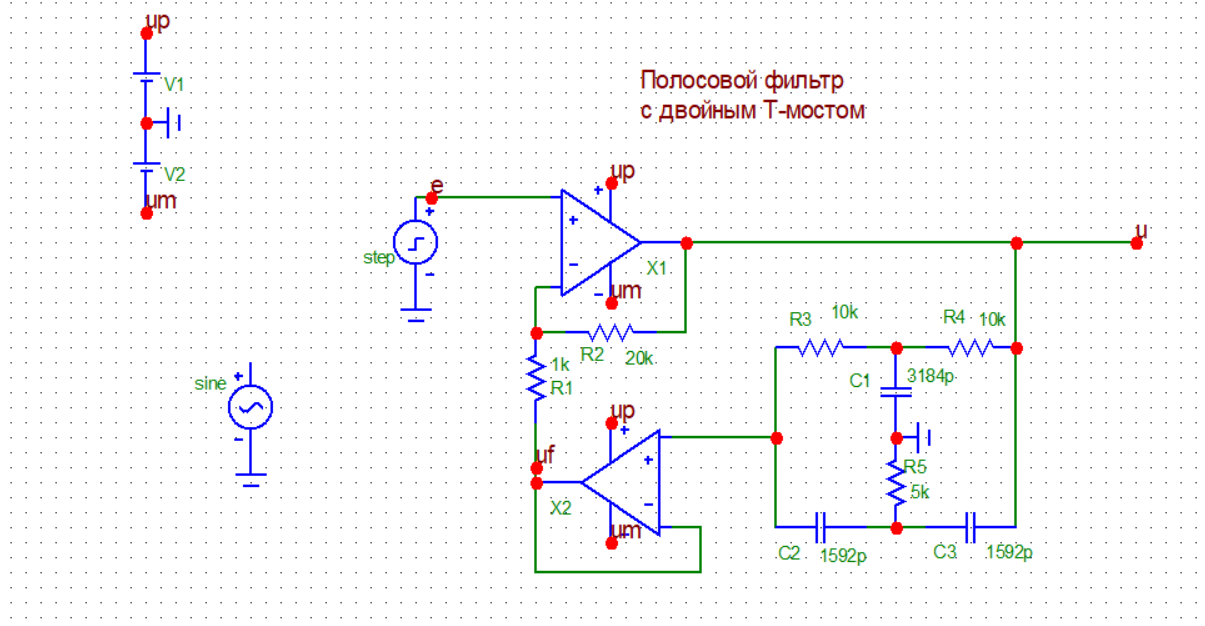
\includegraphics[width=1.0\linewidth]{res/pass2T_scheme.png}
		\caption{Схема}
		\label{scheme}
	\end{figure}
	
	Проварьируем $R_2 = [20k, 100k | 20k]$.

	\begin{figure}[H]
		\centering
		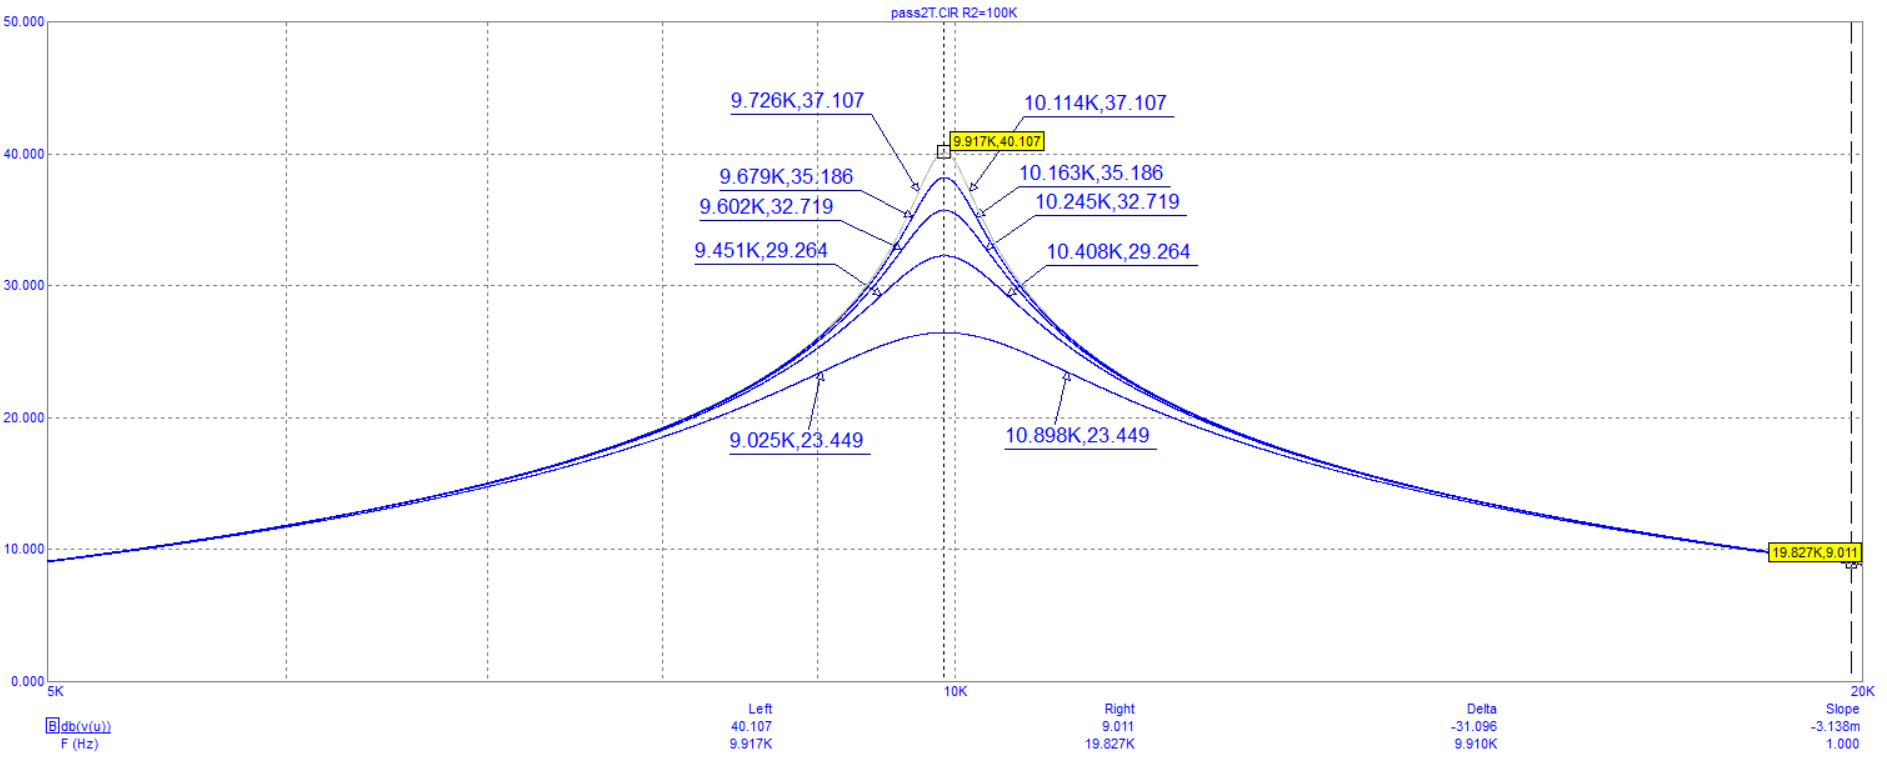
\includegraphics[width=1.0\linewidth]{res/pass2T_R2.png}
		\caption{АЧХ}
		\label{scheme}
	\end{figure}
	
	Изучим поведение фильтра при варьировании $R_5 = [1.5k, 5.5k | 500]$
	Максимум достигается при $R_5 \approx 3k$
	\begin{figure}[H]
		\centering
		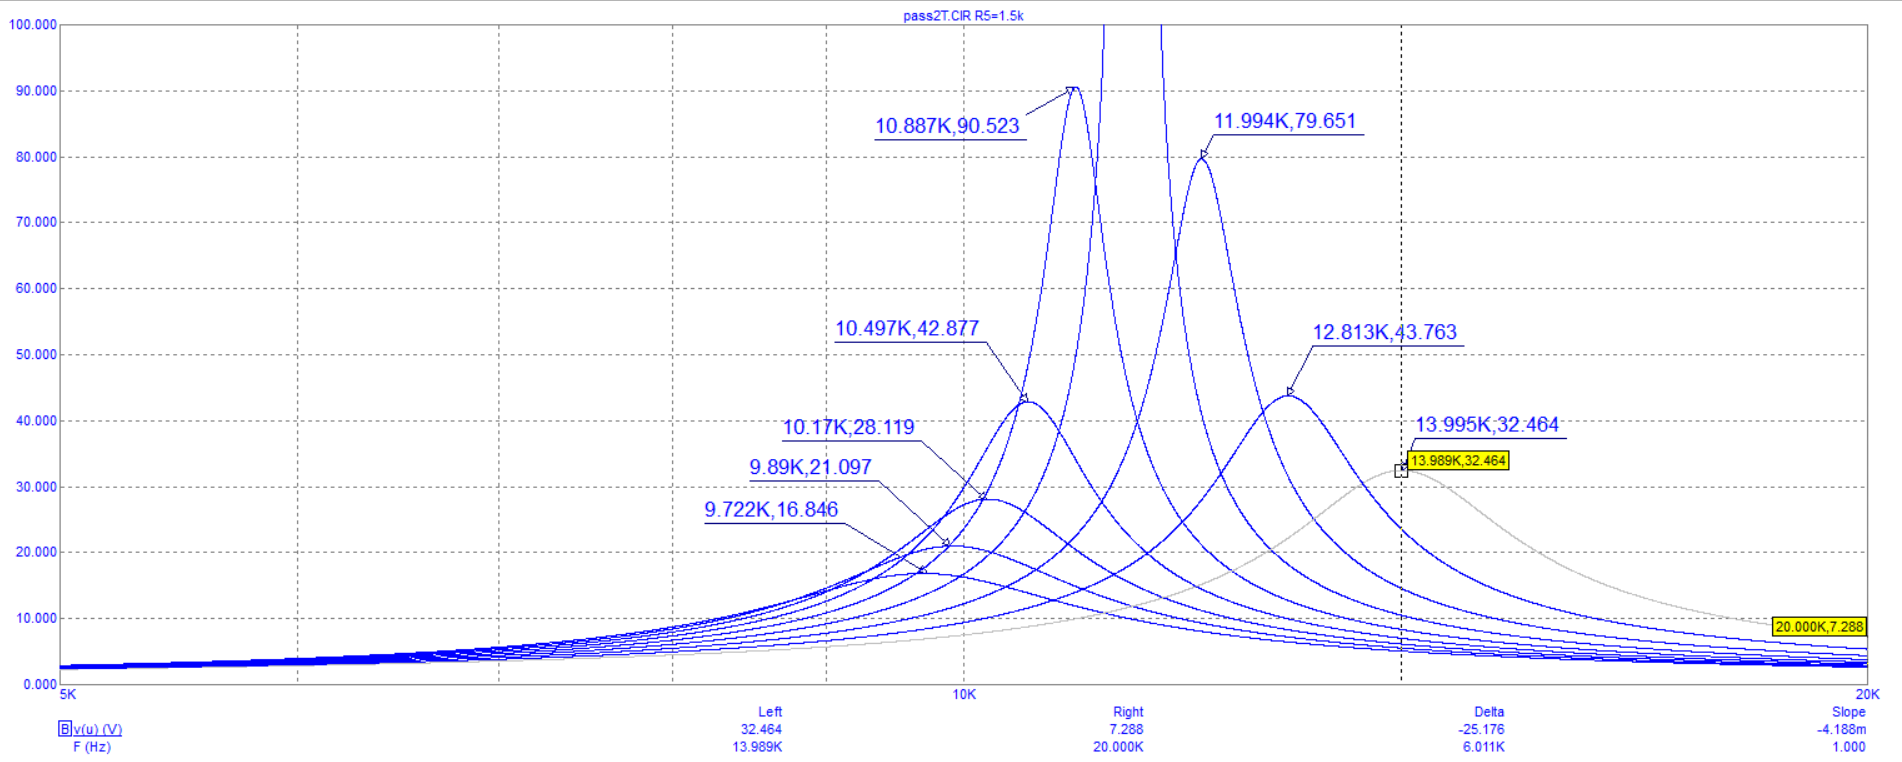
\includegraphics[width=1.0\linewidth]{res/pass2T_R5.png}
		\caption{АЧХ}
		\label{scheme}
	\end{figure}
	
	Рассмотрим переходную характеристику:
	\begin{figure}[H]
		\centering
		\begin{minipage}[b]{.5\textwidth}
			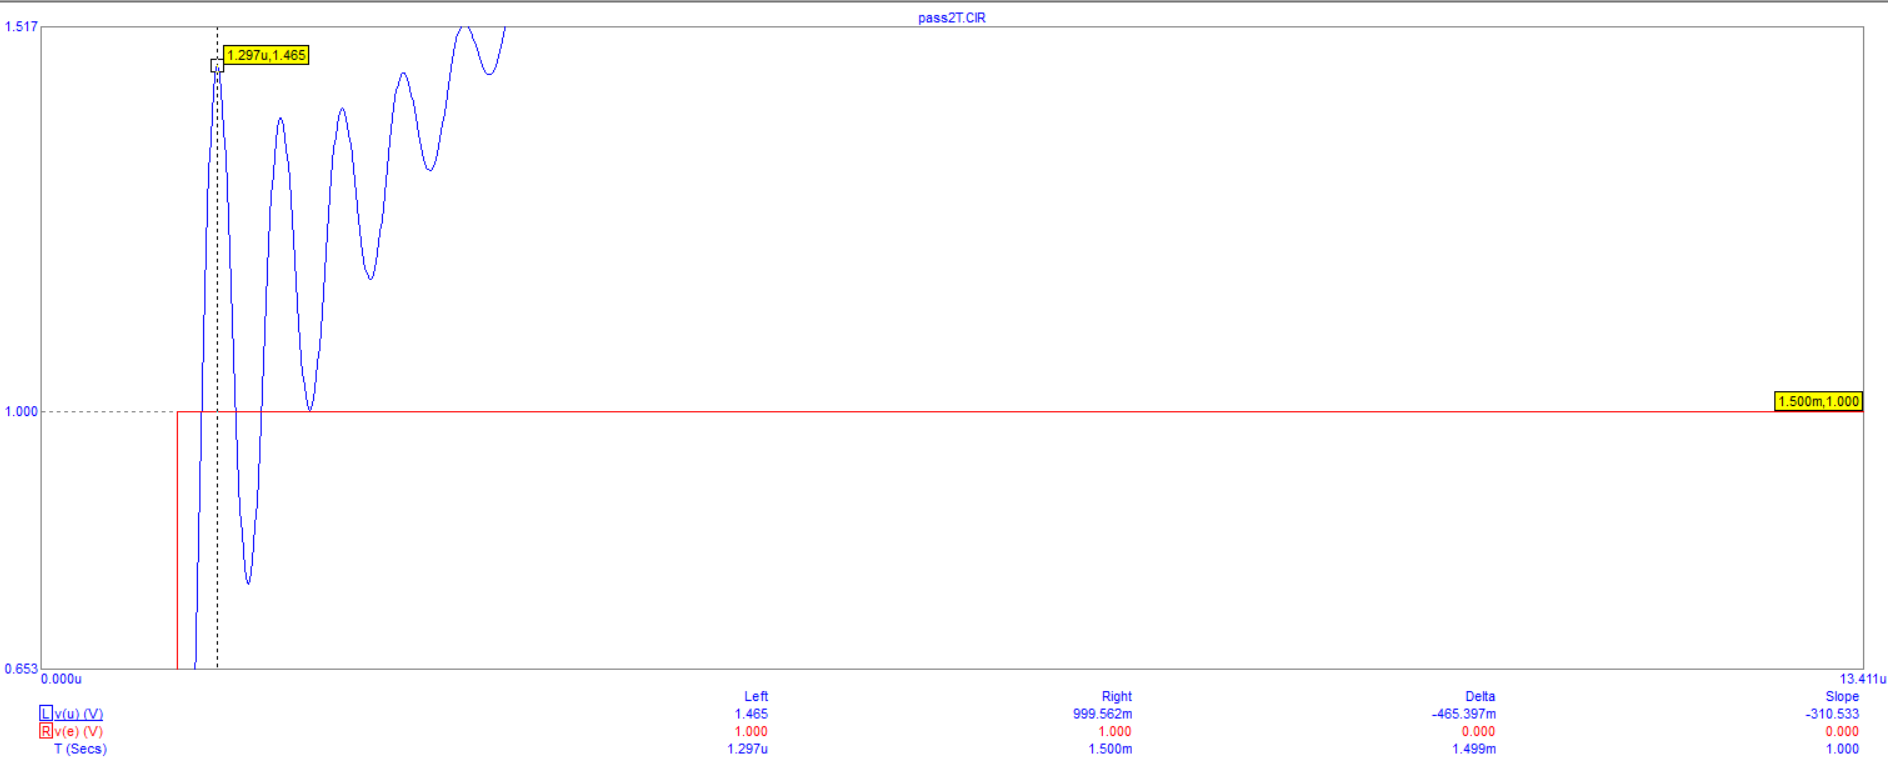
\includegraphics[width=1\linewidth]{res/pass2T_first.png}
		\end{minipage}%
		\begin{minipage}[b]{.5\textwidth}
			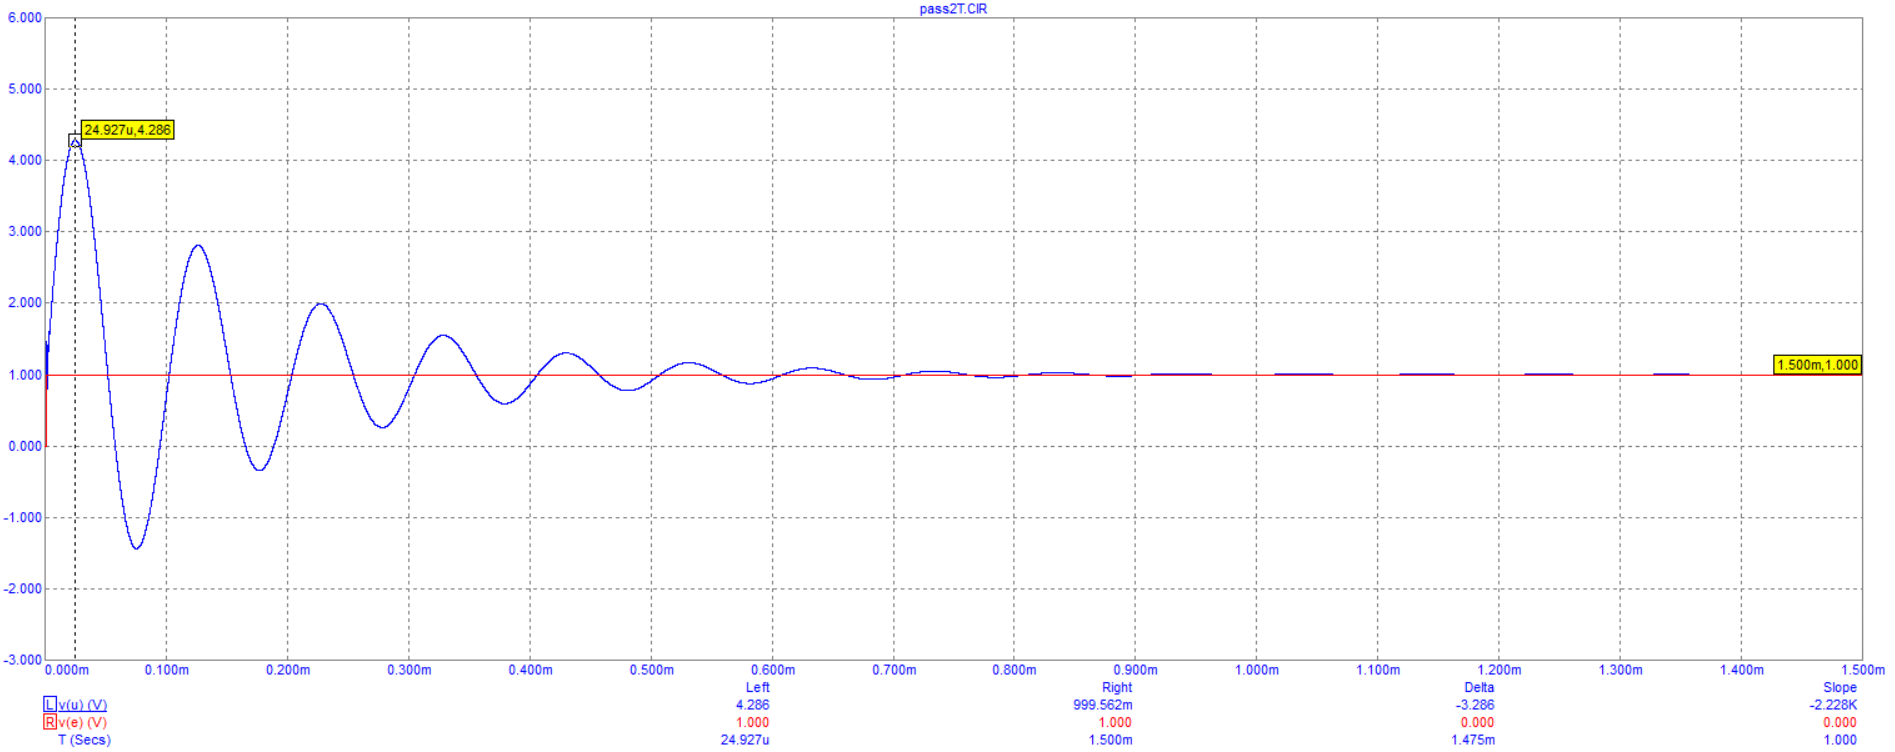
\includegraphics[width=1\linewidth]{res/pass2T_peak.png}
		\end{minipage}
		\caption{Переходная характеристика полосового фильтра}
	\end{figure}
	
	Изучим переходную характеристику при варьировании $R_5 = [5.0k, 2.5k | 500]$.
	Видно, что при $R_5 < 3k$ фильтр устойчив.
	\begin{figure}[H]
		\centering
		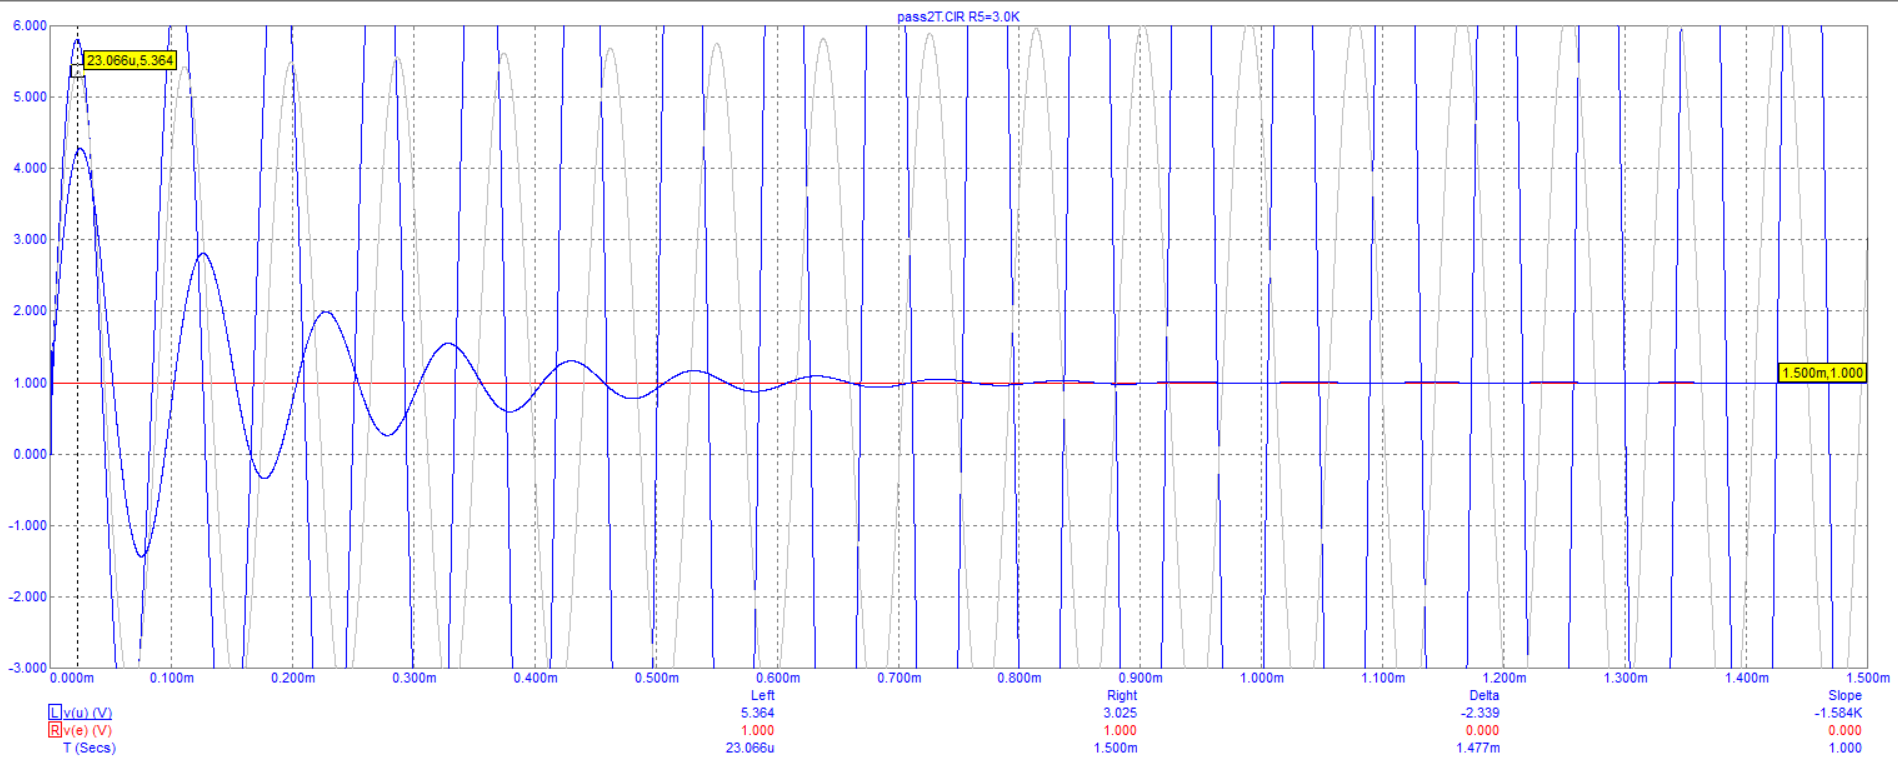
\includegraphics[width=1.0\linewidth]{res/pass2T_R5_transient.png}
		\caption{Переходная характеристика}
		\label{scheme}
	\end{figure}
	
	Изучим модель режекторного фильтра $f_0 = 10k, \gamma = 0.1$.
	\begin{figure}[H]
		\centering
		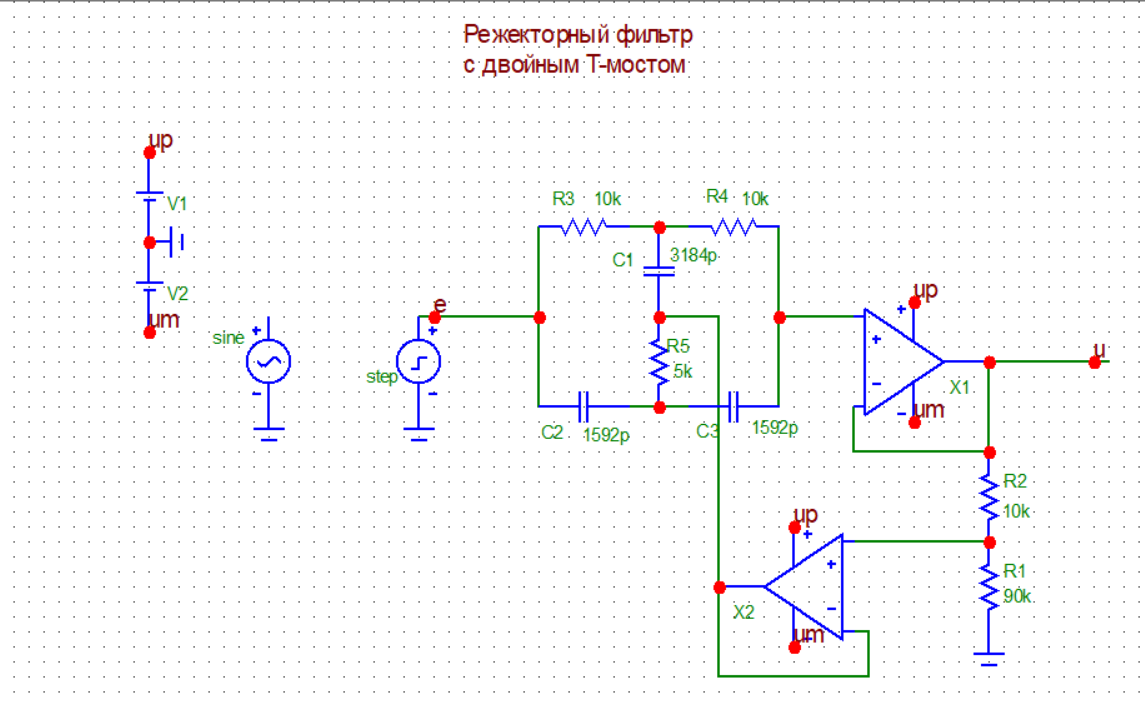
\includegraphics[width=1.0\linewidth]{res/stop2T_scheme.png}
		\caption{Схема}
		\label{scheme}
	\end{figure}
	
	Рассмотрим АЧХ и ФЧХ фильтра.
	\begin{figure}[H]
		\centering
		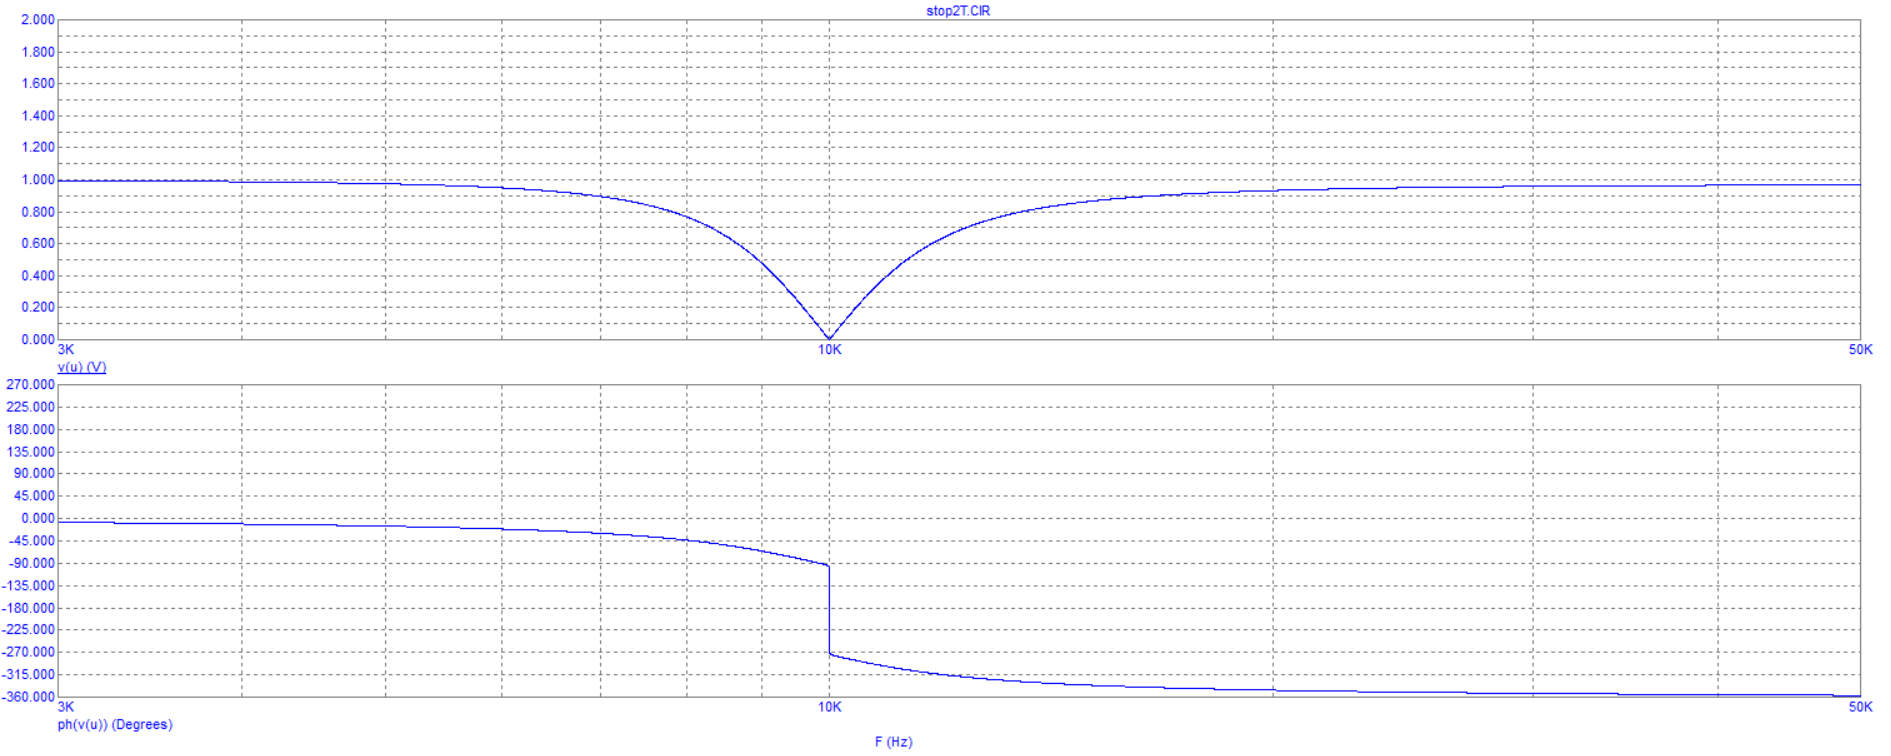
\includegraphics[width=1.0\linewidth]{res/stop2T.png}
		\caption{АЧХ и ФЧХ}
		\label{scheme}
	\end{figure}
	
	Проварьируем $R_1 = [90k, 240k|30k]$. Полоса при $R_1 = 90k$ указана на рисунке.
	\begin{figure}[H]
		\centering
		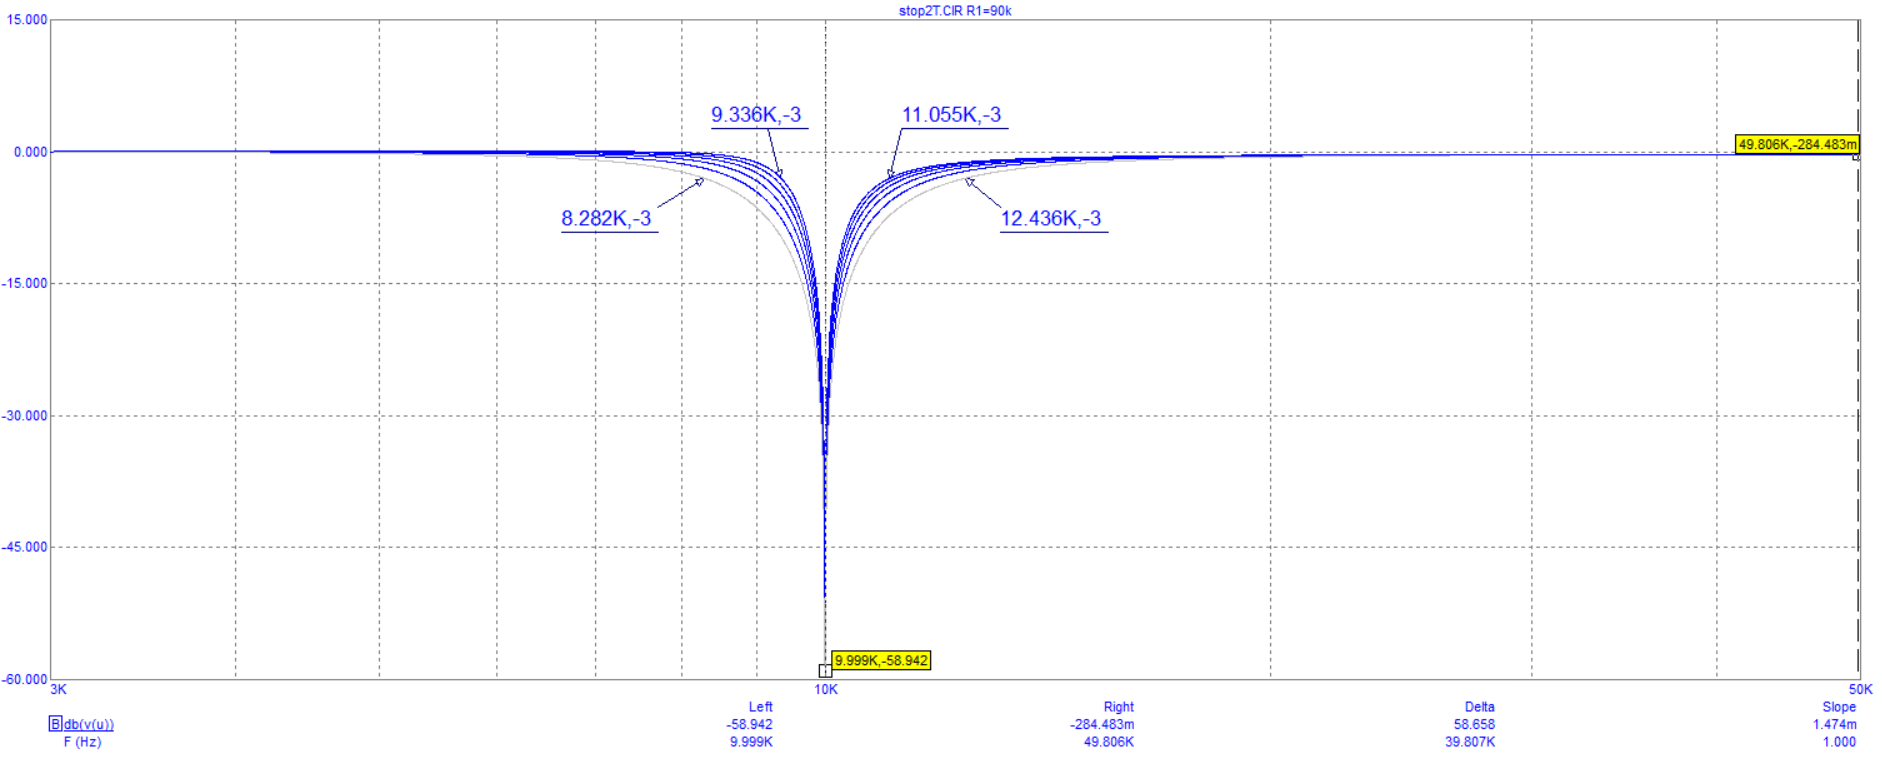
\includegraphics[width=1.0\linewidth]{res/stop2T_R1_90_240.png}
		\caption{АЧХ}
		\label{scheme}
	\end{figure}
	
	Проварьируем $R_1 = [300k, 1500k|300k]$.
	Уровень выброса при $R_1 = 1500k$ указан на рисунке.
	\begin{figure}[H]
		\centering
		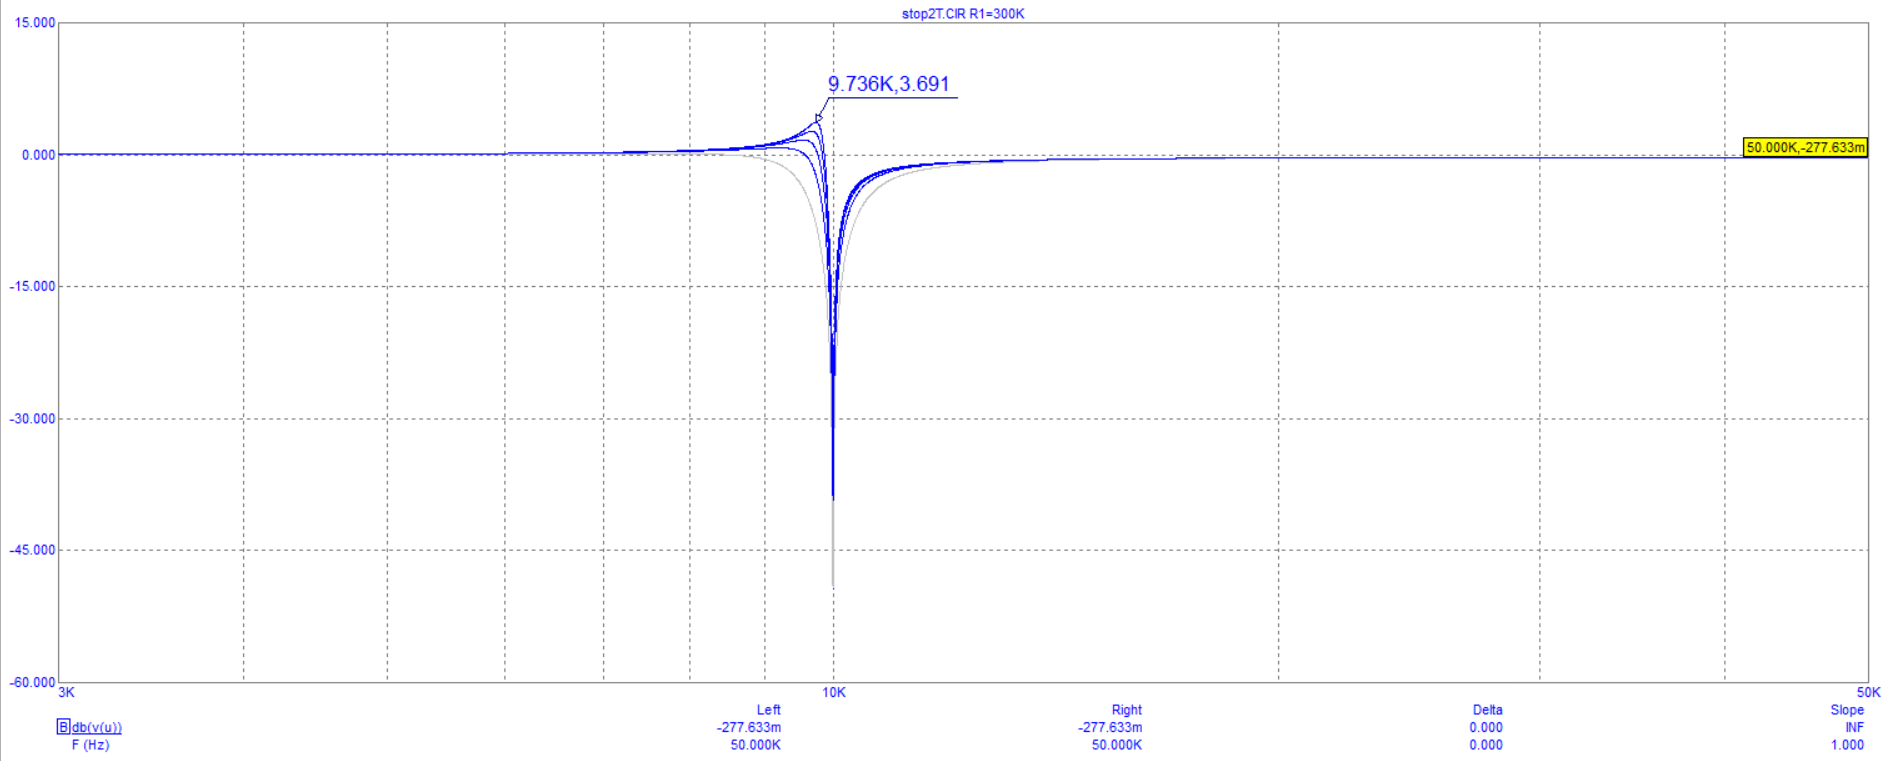
\includegraphics[width=1.0\linewidth]{res/stop2T_R1_300_1500.png}
		\caption{АЧХ}
		\label{scheme}
	\end{figure}
	
	Варьируем $R_5 = [1k, 9k | 2k]$.
	\begin{figure}[H]
		\centering
		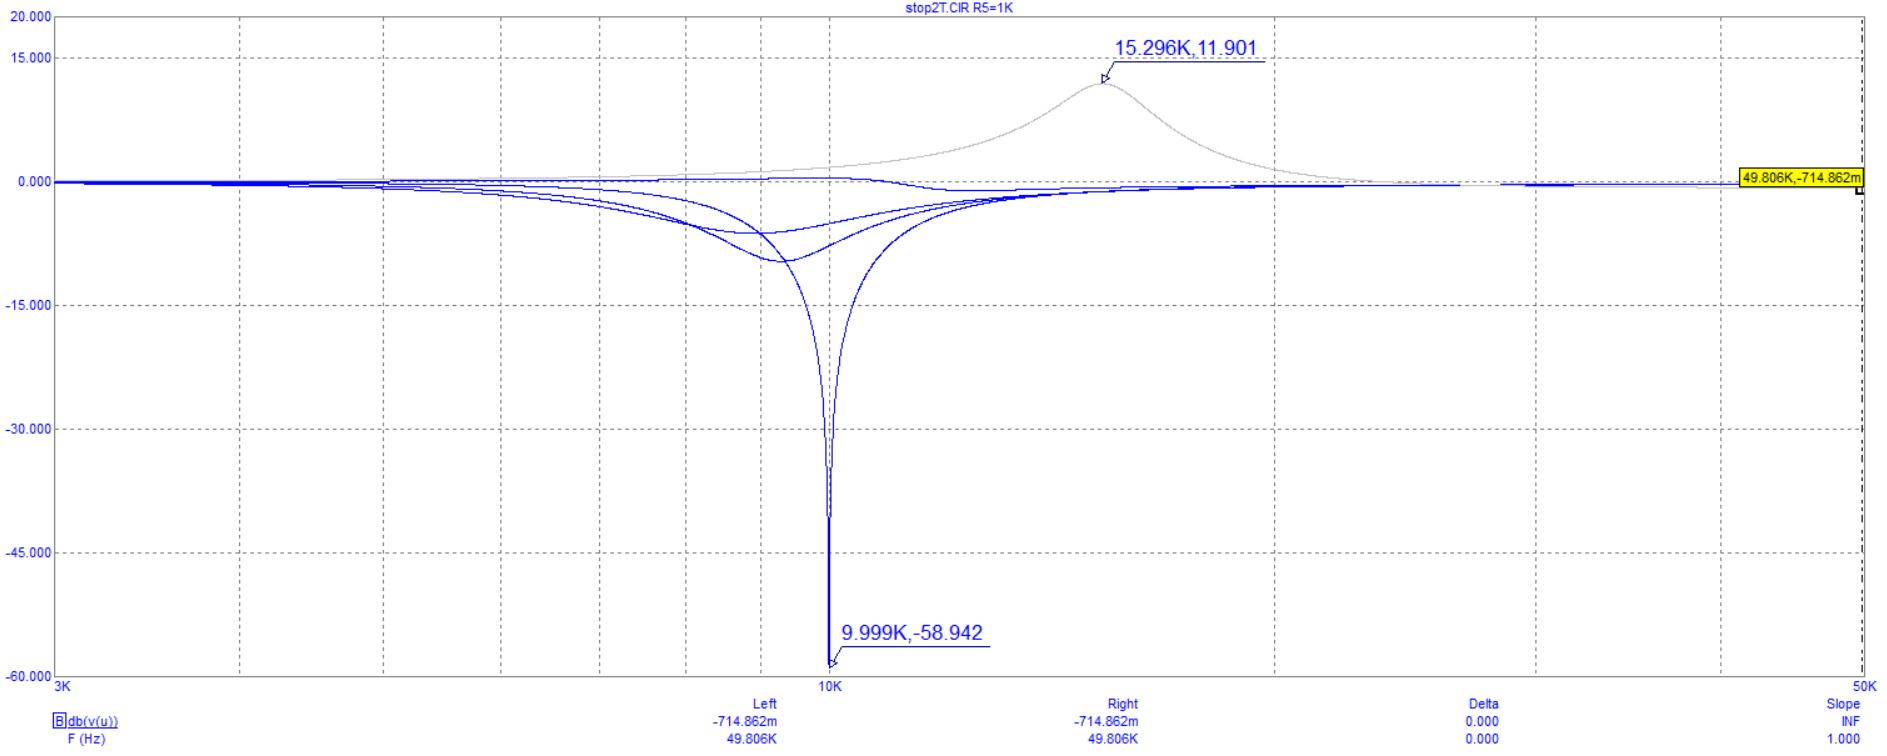
\includegraphics[width=1.0\linewidth]{res/stop2T_R5.png}
		\caption{АЧХ}
		\label{scheme}
	\end{figure}

	Рассмотрим переходную характеристику фильтра.
	Уровни выброса и скачка в нуле указаны на рисунке.
	\begin{figure}[H]
		\centering
		\begin{minipage}[b]{.5\textwidth}
			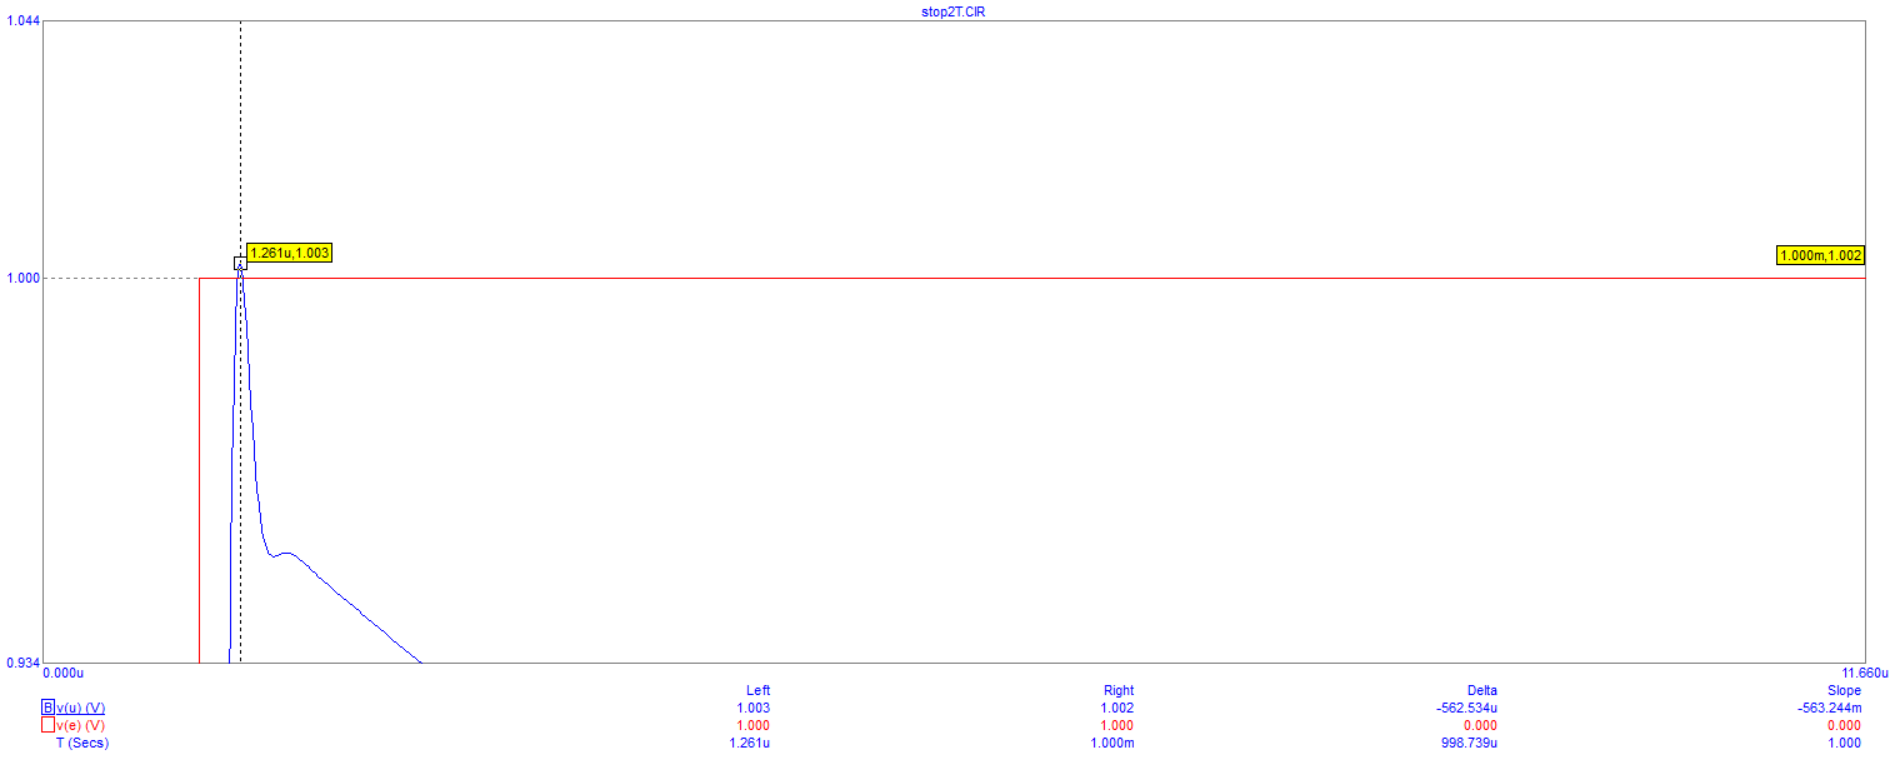
\includegraphics[width=1\linewidth]{res/stop2T_first.png}
		\end{minipage}%
		\begin{minipage}[b]{.5\textwidth}
			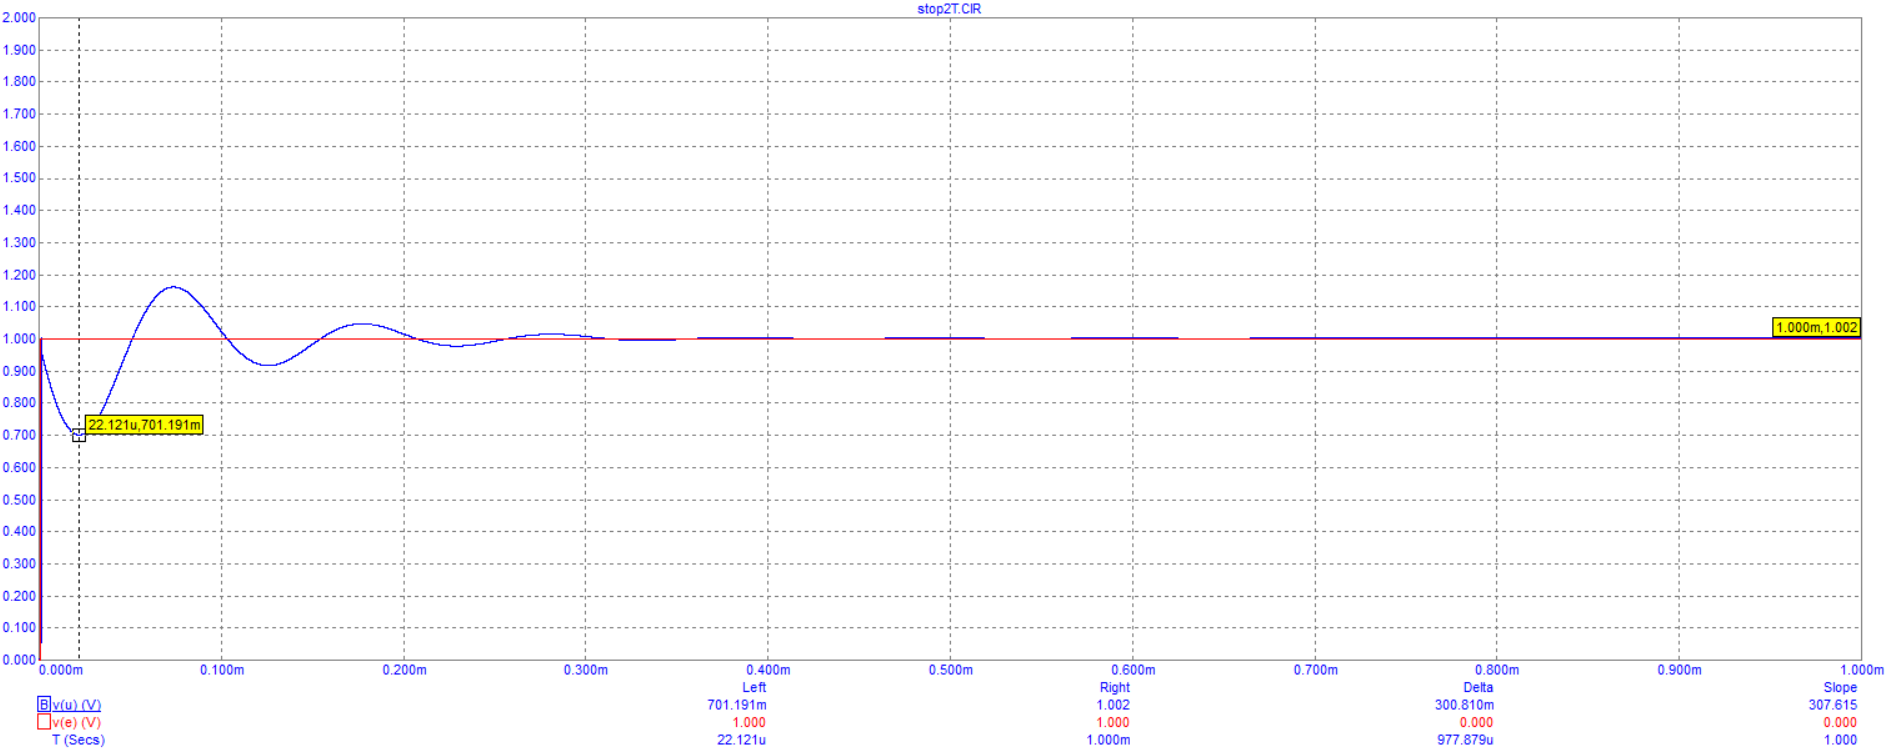
\includegraphics[width=1\linewidth]{res/stop2T_peak.png}
		\end{minipage}
		\caption{Переходная характеристика режекторного фильтра}
	\end{figure}
	
	\section*{9.4 Звенья Саллена-Ки}
	
	Рассмотрим схемы звеньев Саллена-Ки с $f_0 = 10k$, $Q = 1$.
	В них используются неинвертирующие усилители $K = 1 + \frac{R_2}{R_1}$.

	При $f = f_0$ $K = 2$.

	\begin{figure}[H]
		\centering
		\begin{minipage}[b]{0.33\textwidth}
			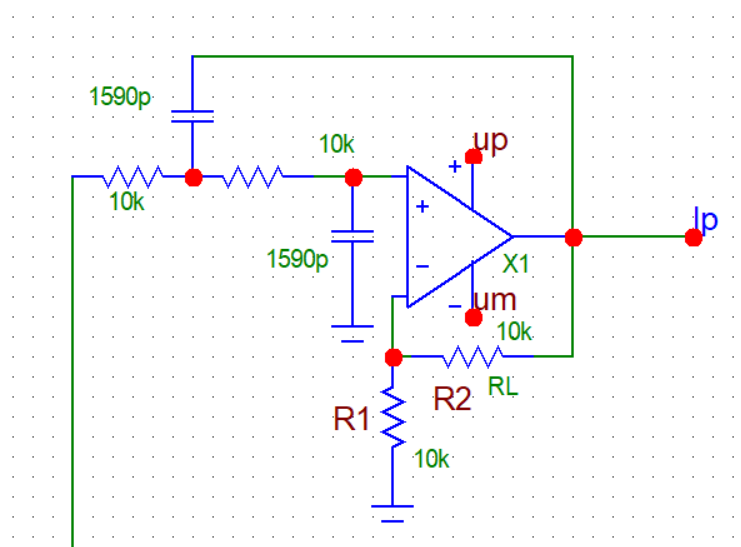
\includegraphics[width=1\linewidth]{res/skey_scheme_lp.png}
		\end{minipage}%
		\begin{minipage}[b]{0.33\textwidth}
			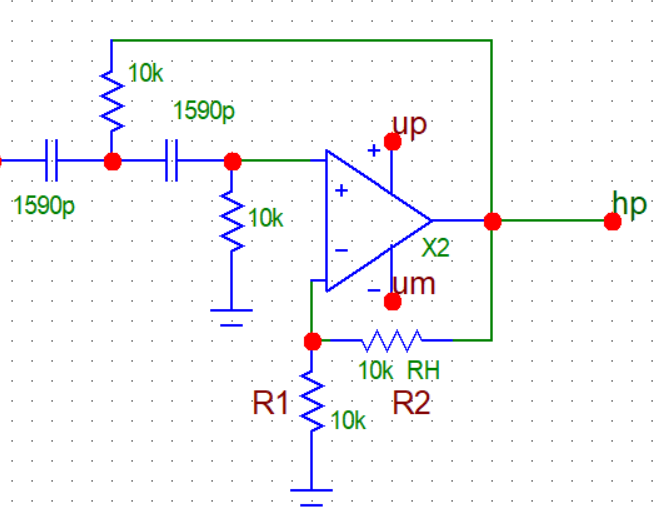
\includegraphics[width=1\linewidth]{res/skey_scheme_hp.png}
		\end{minipage}%
		\begin{minipage}[b]{0.33\textwidth}
			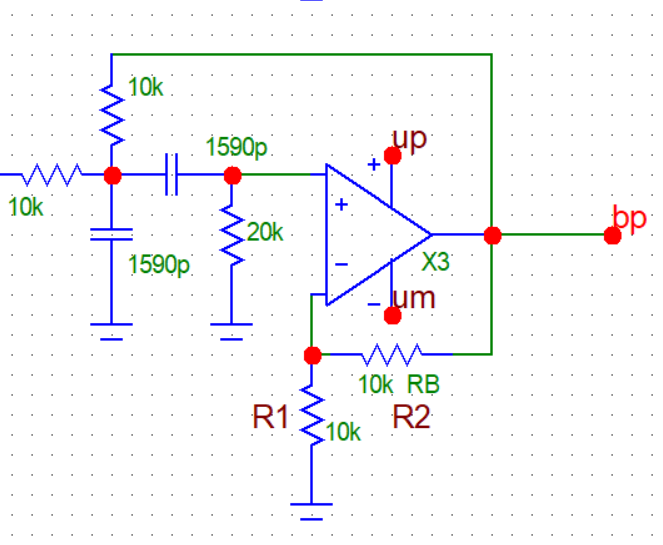
\includegraphics[width=1\linewidth]{res/skey_scheme_bp.png}
		\end{minipage}
		\caption{Схемы}
	\end{figure}
	
	\begin{figure}[H]
		\centering
		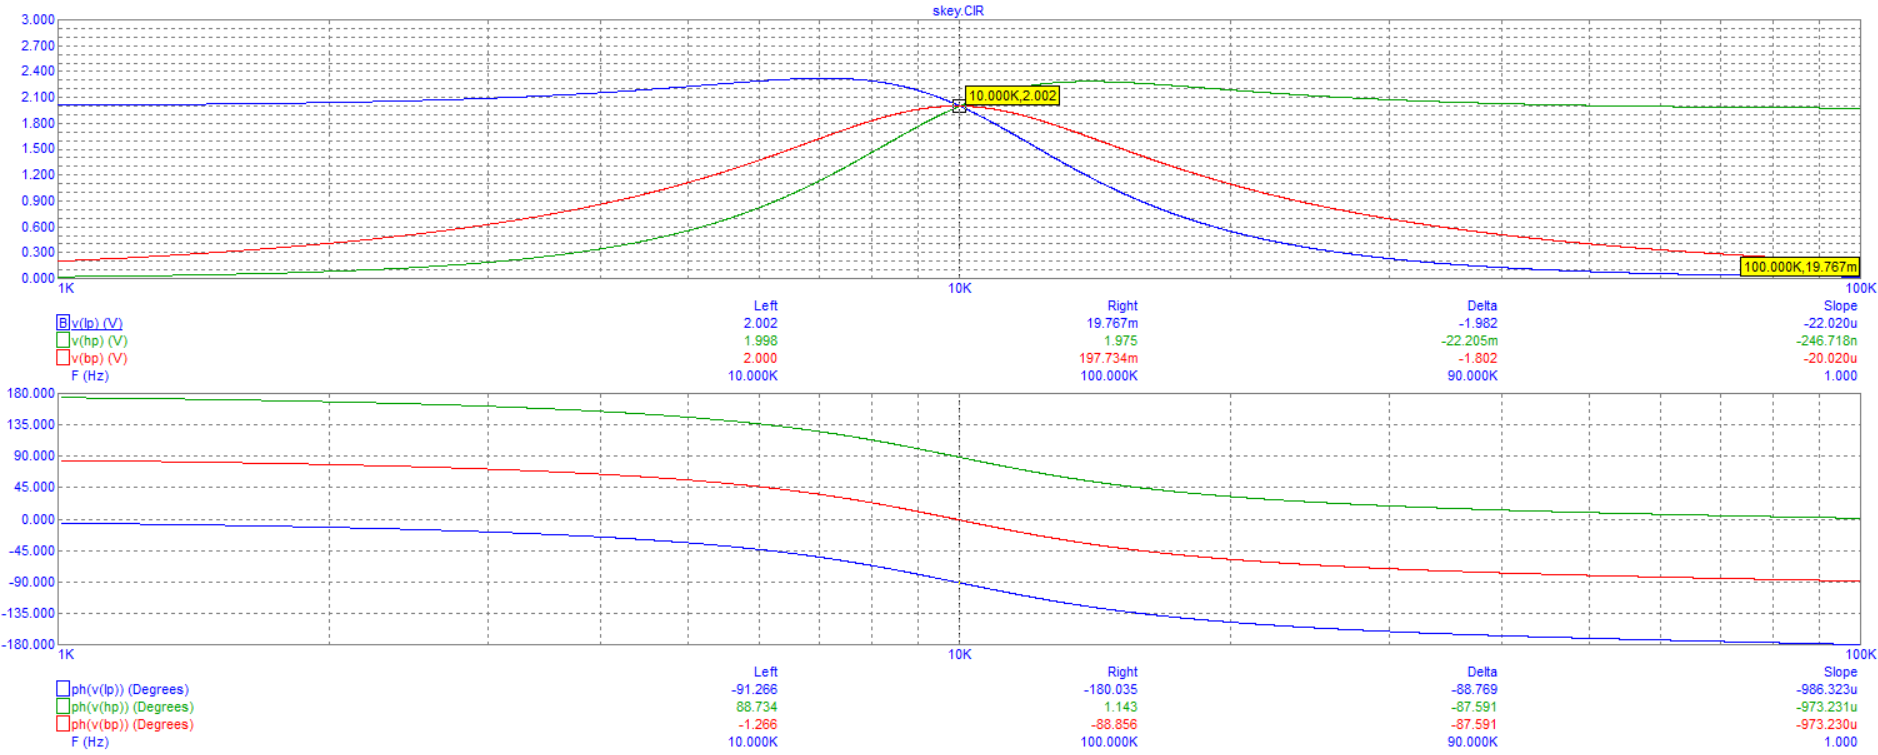
\includegraphics[width=1.0\linewidth]{res/skey.png}
		\caption{АЧХ и ФЧХ звеньев Саллена-Ки}
		\label{scheme}
	\end{figure}
	
	Проварьируем $R_L, R_H, R_B = [11k, 19k | 2k]$.
	\begin{figure}[H]
		\centering
		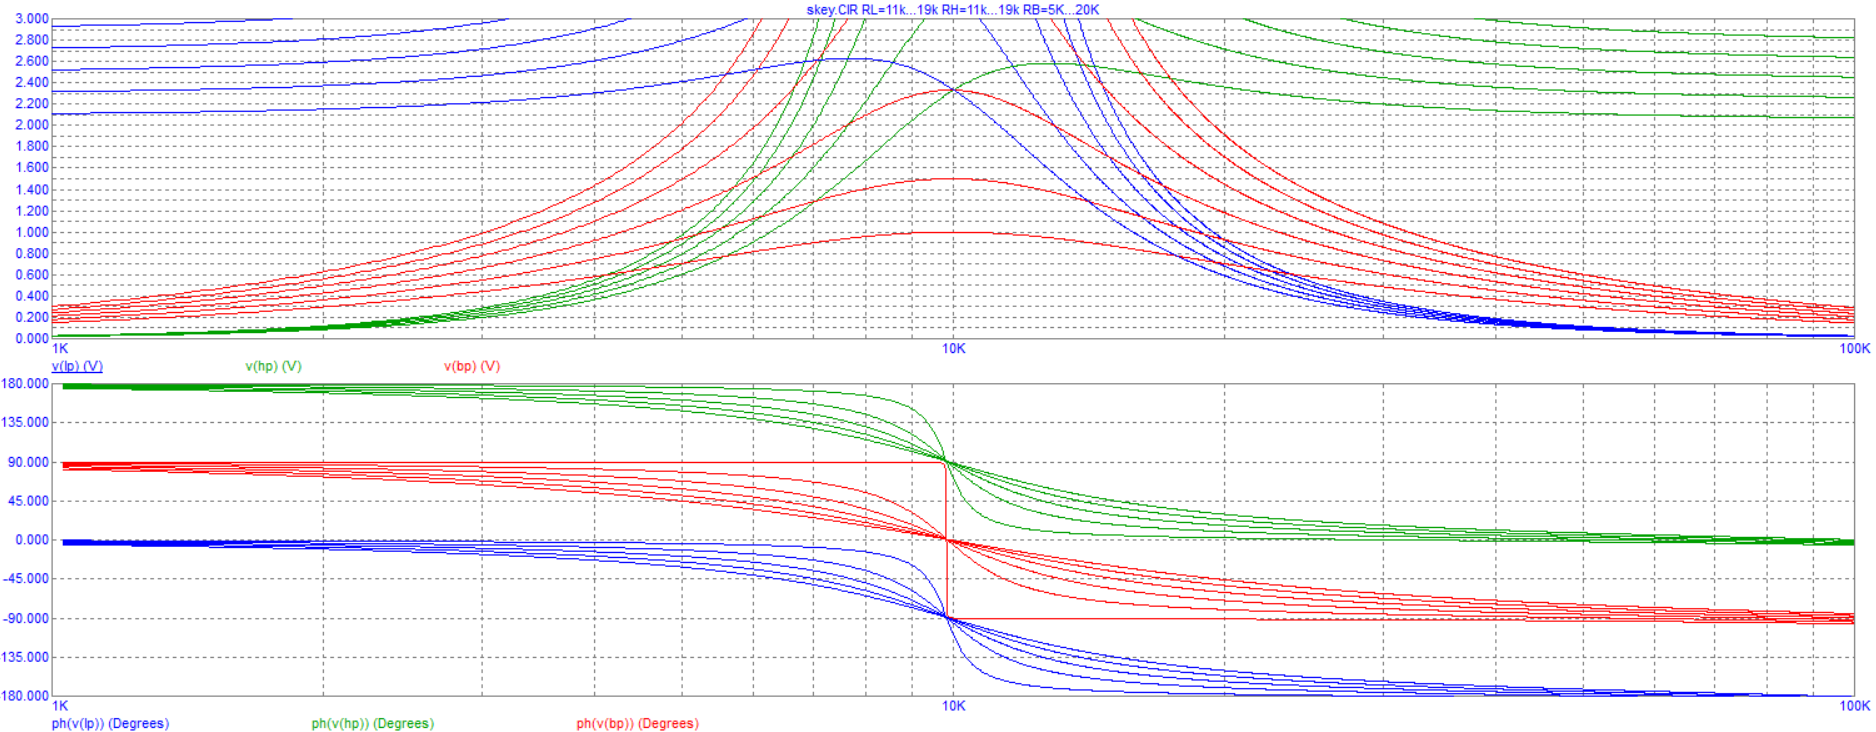
\includegraphics[width=1.0\linewidth]{res/skey_11_19.png}
		\caption{АЧХ и ФЧХ звеньев Саллена-Ки}
		\label{scheme}
	\end{figure}

	Пиковые значения усиления составляют $K_{lp} = 29.441$, $K_{hp} = 28.320$, $K_{bp} = 28.860$.
	\begin{figure}[H]
		\centering
		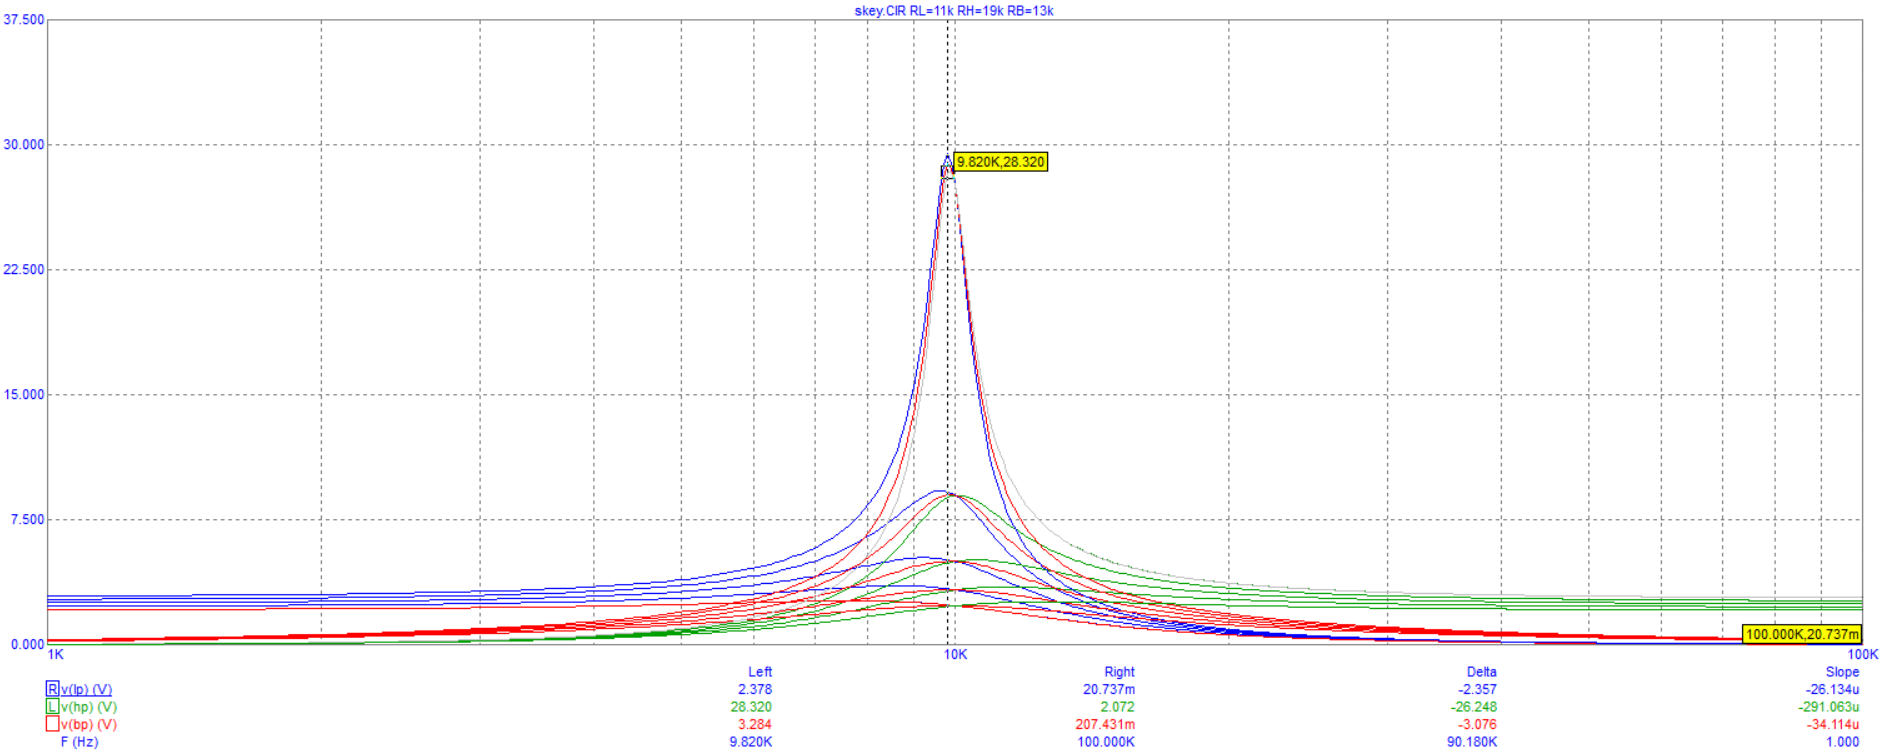
\includegraphics[width=1.0\linewidth]{res/skey_11_19_scoped.png}
		\caption{АЧХ звеньев Саллена-Ки}
		\label{scheme}
	\end{figure}
	
	Переходная характеристика звеньев:
	\begin{itemize}
		\item Звено низких частот имеет нулевую производную в нуле, а также устанавливается в ненулевом положении.
		\item Звено высоких частот имеет скачок в нуле и стремится к нулю с течением времени.
		\item Полосовой фильтр не имеет скачка в нуле и стремится к нулю с течением времени.
	\end{itemize}

	\begin{figure}[H]
		\centering
		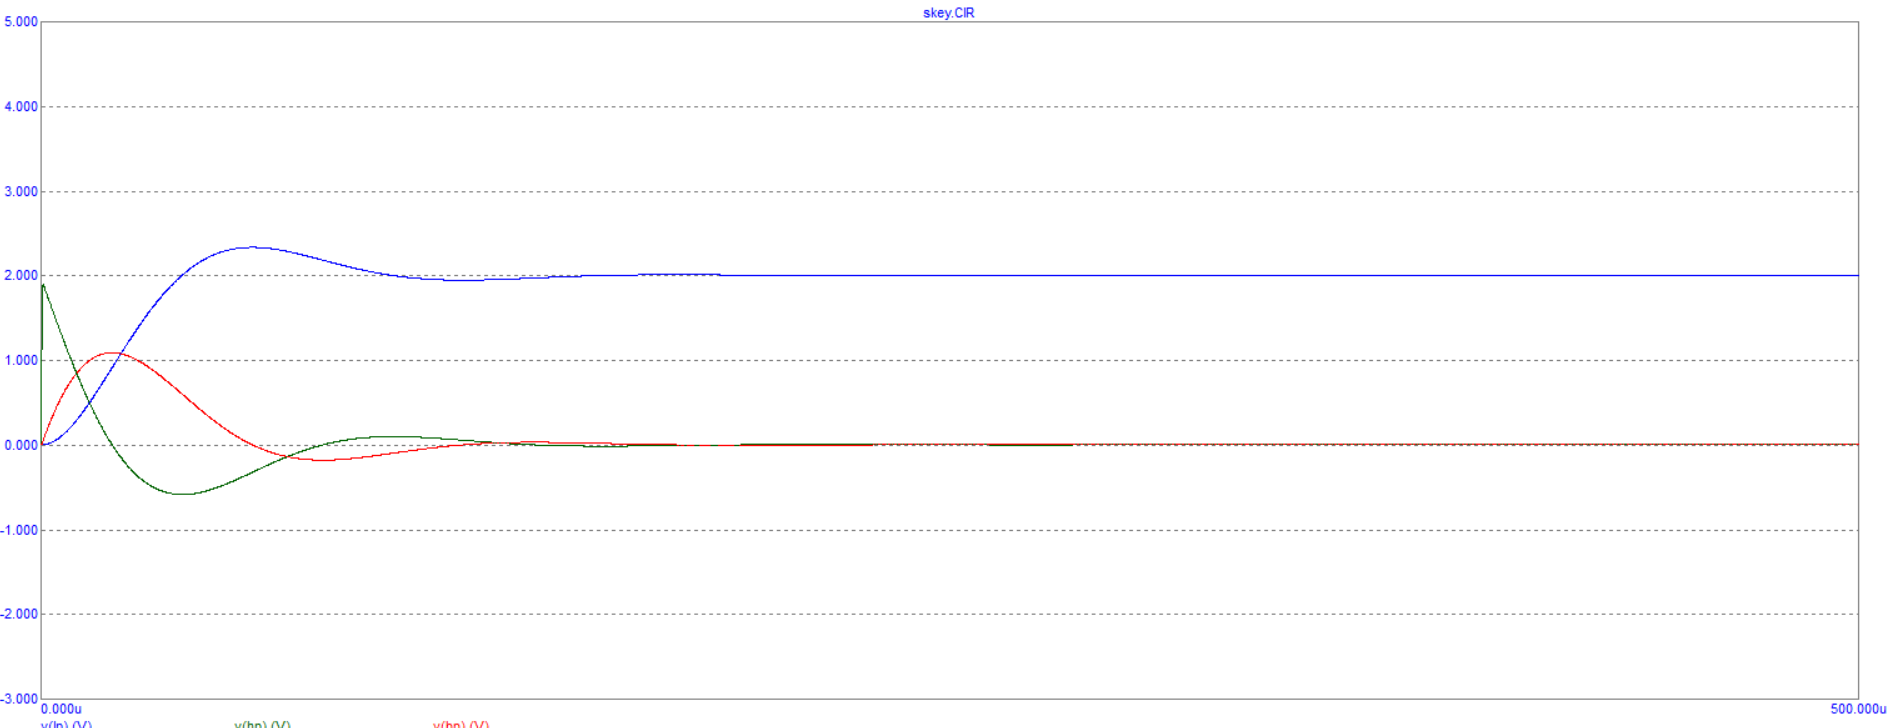
\includegraphics[width=1.0\linewidth]{res/skey_transient.png}
		\caption{Переходная характеристика звеньев Саллена-Ки}
		\label{scheme}
	\end{figure}
	Проварьируем $R_L, R_H, R_B = [11k, 19k | 2k]$.
	\begin{figure}[H]
		\centering
		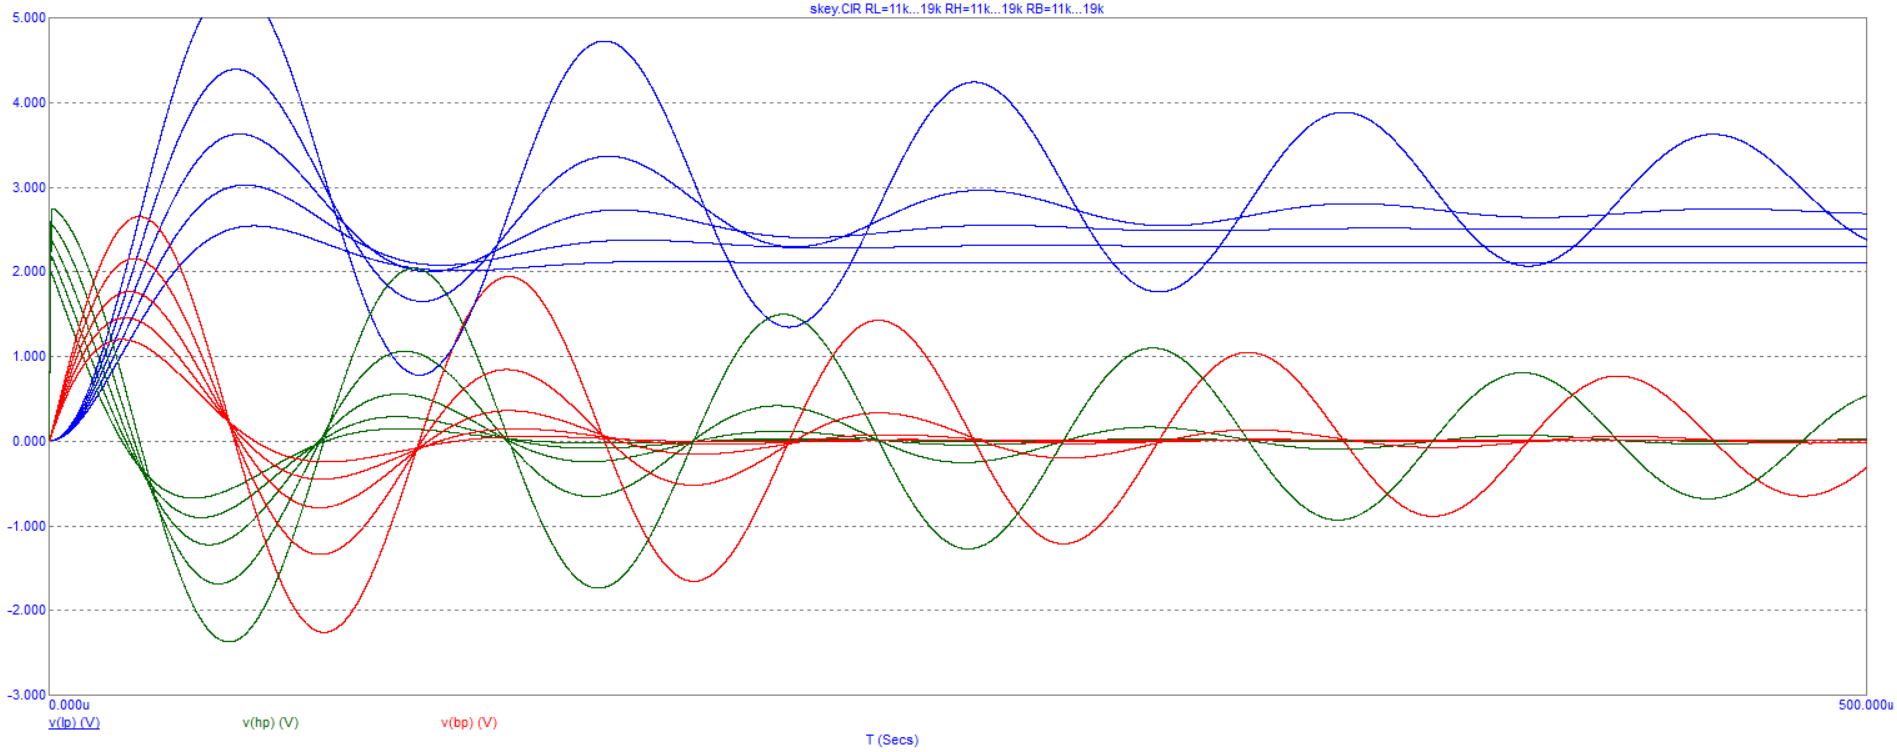
\includegraphics[width=1.0\linewidth]{res/skey_transient_11_19.png}
		\caption{Переходная характеристика при варьировании}
		\label{scheme}
	\end{figure}
	
	Изучим ФВЧ и ФНЧ Баттерворта $n = 3$ на $f_0 = 10k$.
	Одиночные вещественные полюсы реализованы интегрирующей и дифференцирующей цепочками.
	Сопряженные пары -- звеньями Саллена-Ки с добротностью $Q = 1$.
	\begin{figure}[H]
		\centering
		\begin{minipage}[b]{.5\textwidth}
			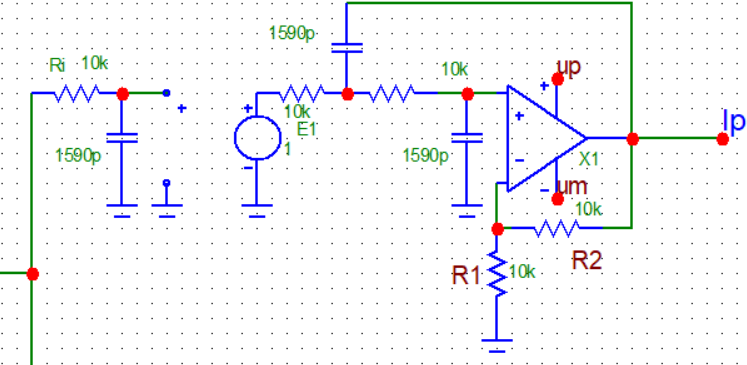
\includegraphics[width=1\linewidth]{res/sk3pole_scheme_lp.png}
		\end{minipage}%
		\begin{minipage}[b]{.5\textwidth}
			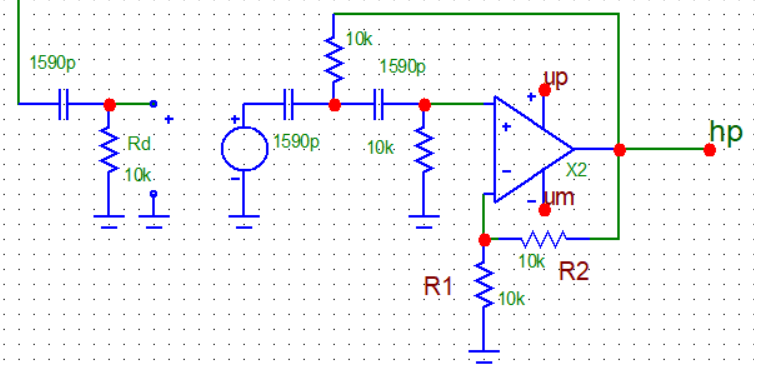
\includegraphics[width=1\linewidth]{res/sk3pole_scheme_hp.png}
		\end{minipage}
		\caption{Схемы}
	\end{figure}
	
	Затухание составляет $60$ dB/декаду.
	\begin{figure}[H]
		\centering
		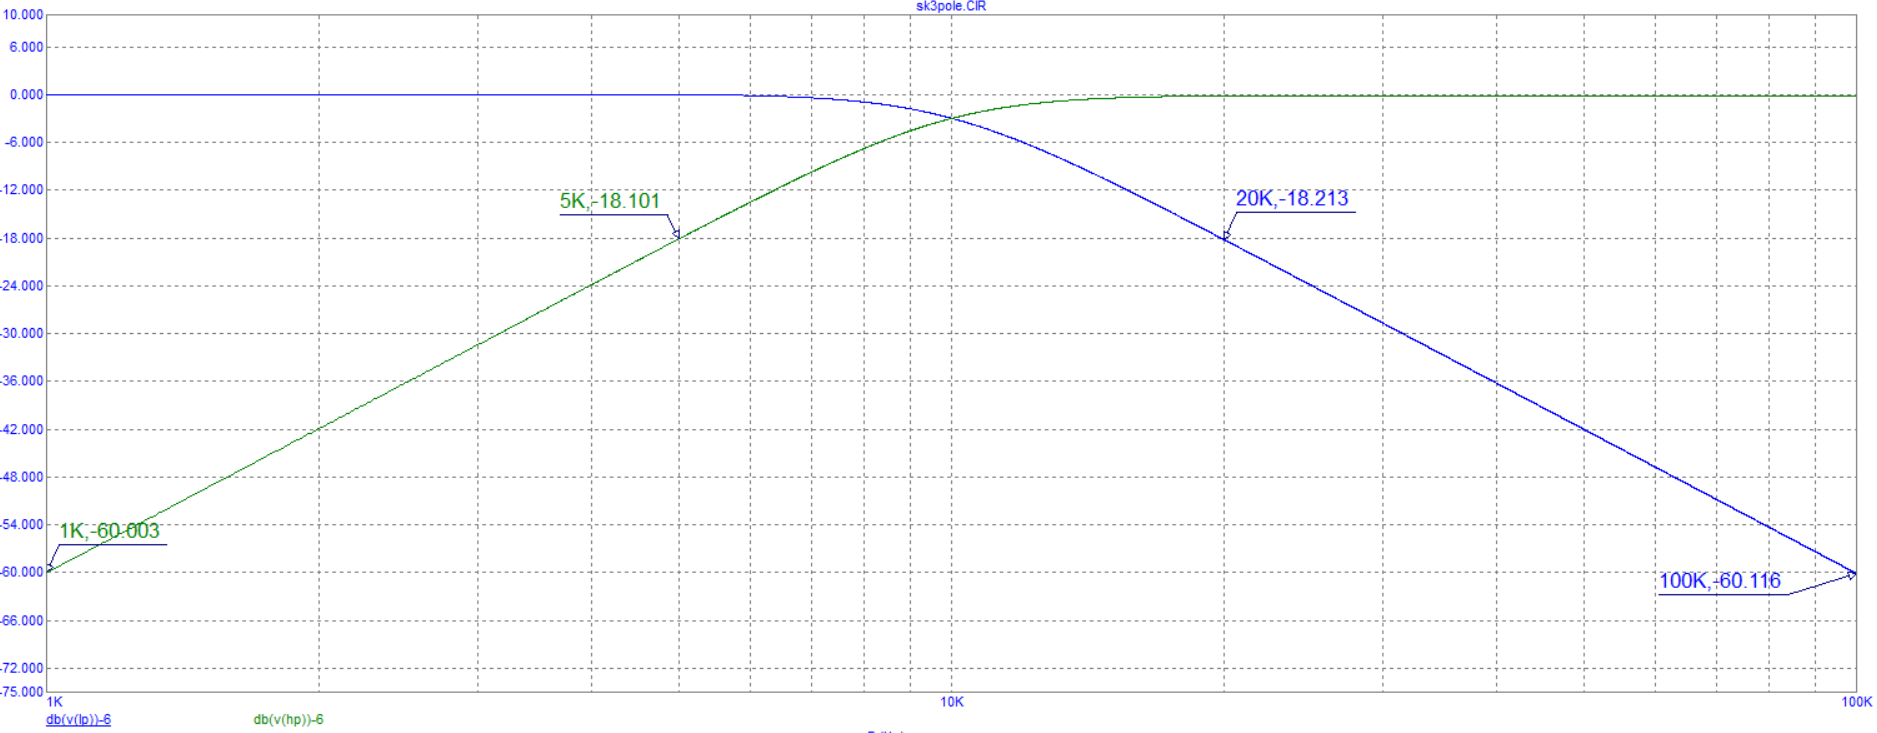
\includegraphics[width=1.0\linewidth]{res/sk3pole_ach.png}
		\caption{АЧХ фильтров Баттерворта}
		\label{scheme}
	\end{figure}
	
	Преобразуем схемы в фильтры Чебышева с $\varepsilon = 1$. Параметры ФНЧ $[\nu_0 = 0.298, (\nu, Q) = (0.916, 3.073)]$, ФВЧ $[\nu_0 = 3.355, (\nu, Q) = (1.092, 3.073)]$ получим из $MatLab$.
	
	Рассчитаем $R_i = \frac{10k}{\nu_0} = 33.5k$, $R_d = \frac{10k}{\nu_0} = 2.98k$.
	Установим оба резистора фильтра Саллена-Ки $R = \frac{10k}{\nu} = 10.9k$, $R = \frac{10k}{\nu} = 9.2k$. Добротность подстроим резисторами $R_1, R_2$: $R_2 = R_1 (2 - \frac{1}{Q}) = 16.7k$.

	Затухание составляет $62.5$ dB/декаду.
	\begin{figure}[H]
		\centering
		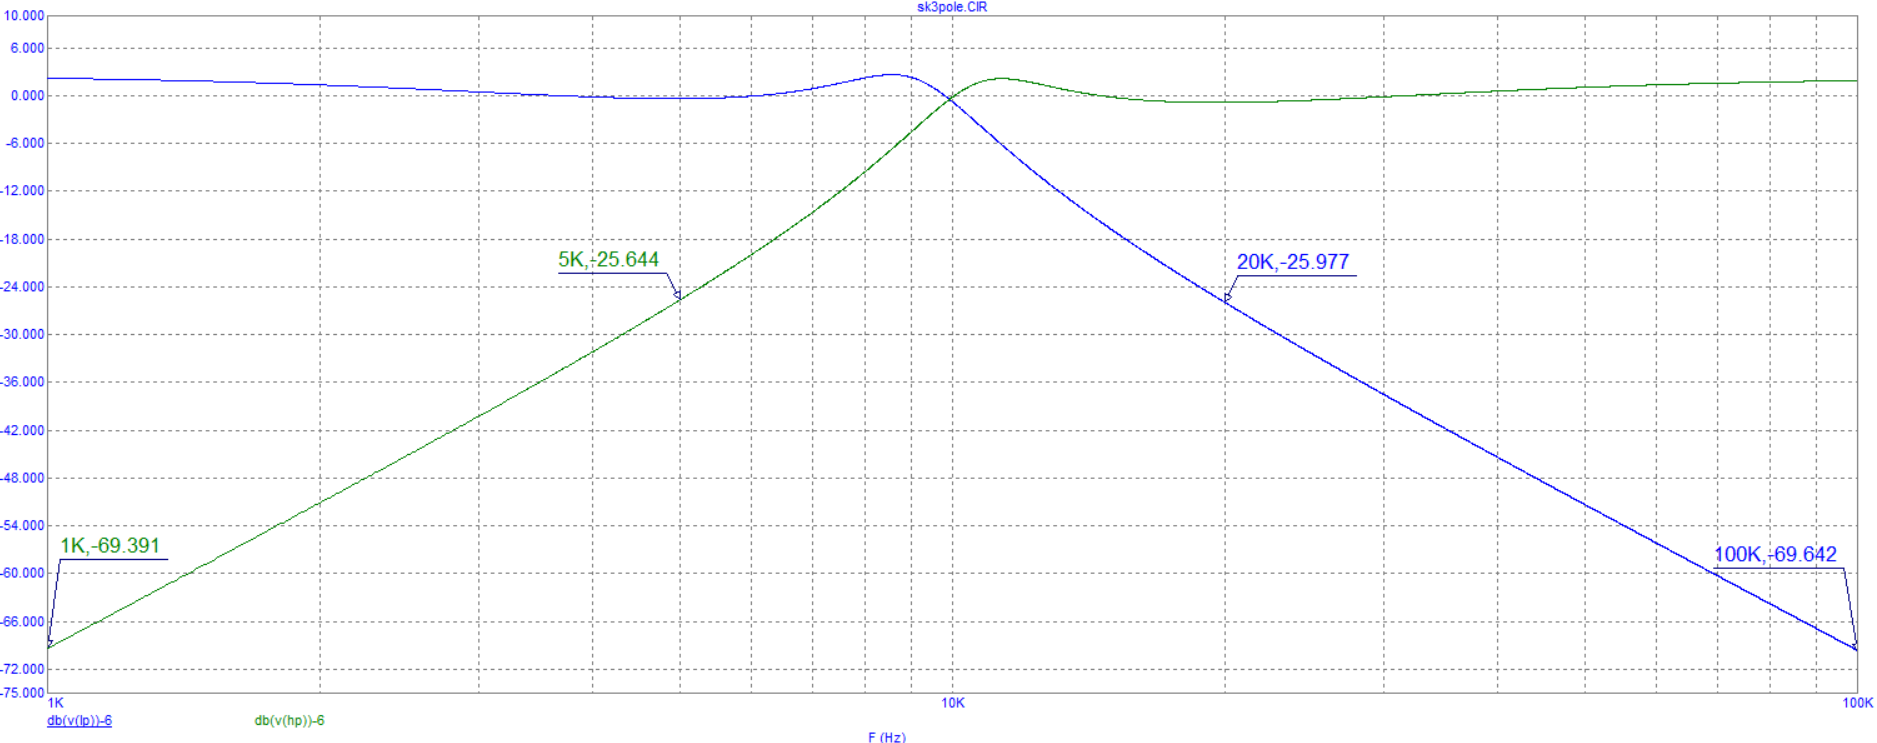
\includegraphics[width=1.0\linewidth]{res/sk3pole_cheb.png}
		\caption{АЧХ фильтров Чебышева}
		\label{scheme}
	\end{figure}

	Построим также фильтр Чебышева второго порядка с $f_0 = 10k$, $\varepsilon = 1$, $Q = \frac{f_0}{\Delta f} = 6$.
	
	\begin{figure}[H]
		\centering
		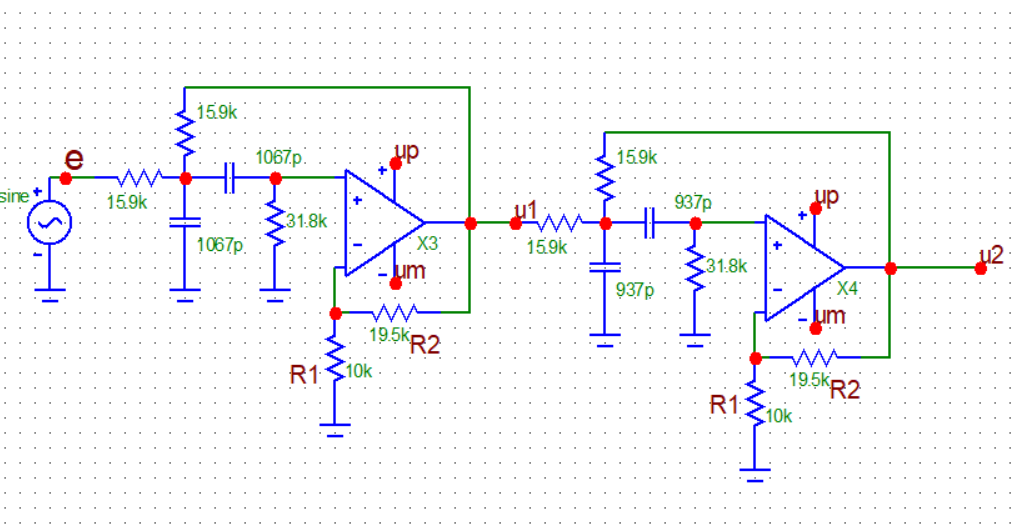
\includegraphics[width=1.0\linewidth]{res/sk4pole_scheme.png}
		\caption{Схема}
		\label{scheme}
	\end{figure}
	
	Как видно из АЧХ, ширина полосы $\Delta f = 1.65k$, значения затухания указаны на рисунке.
	\begin{figure}[H]
		\centering
		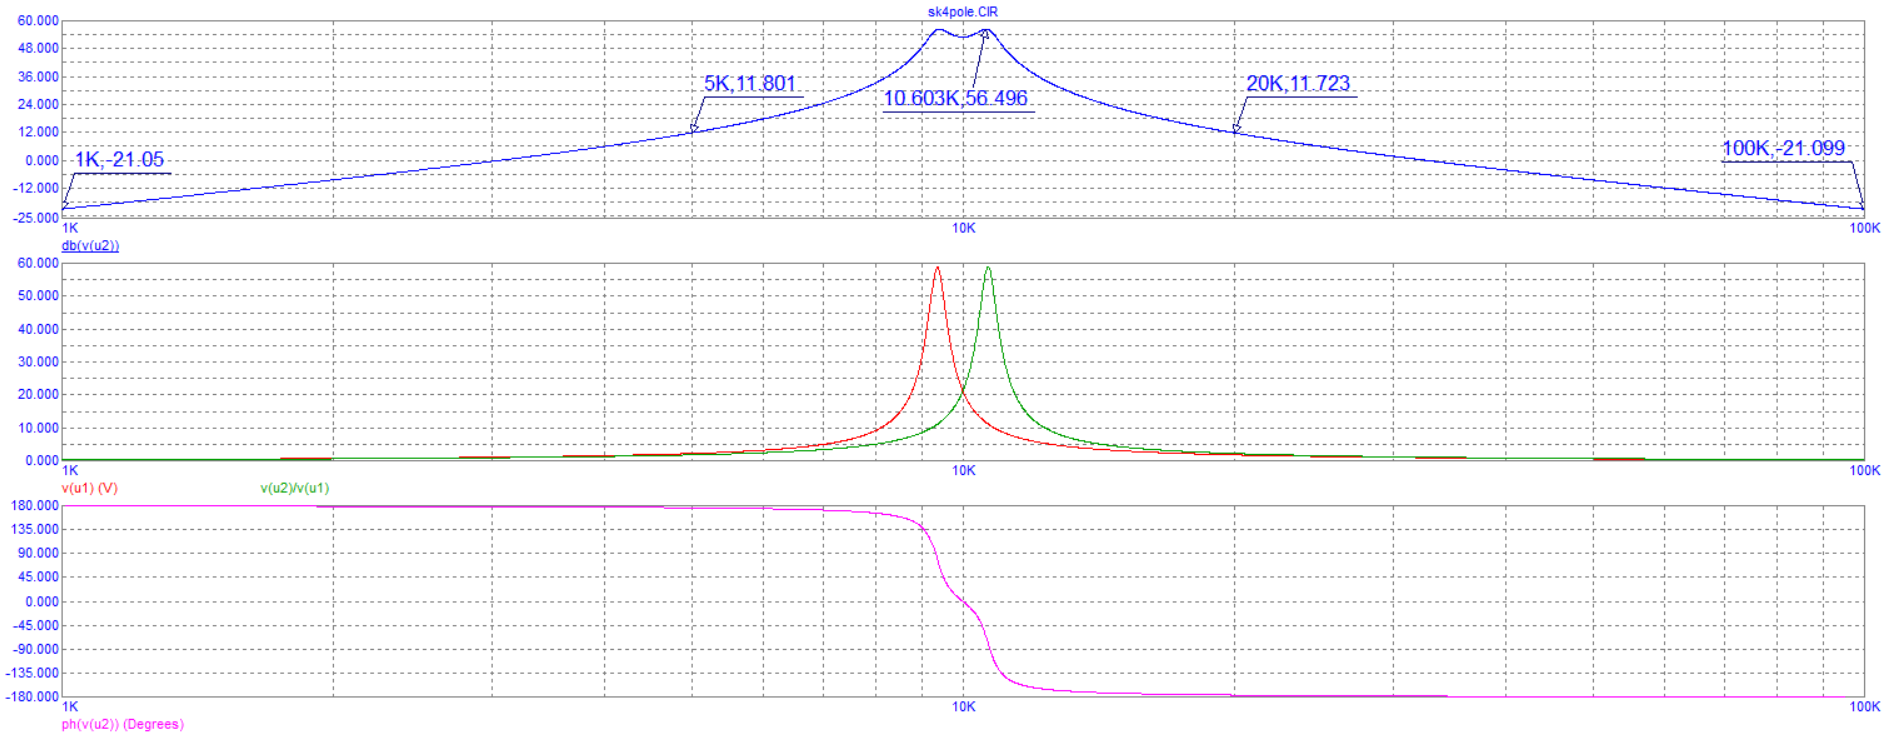
\includegraphics[width=1.0\linewidth]{res/sk4pole.png}
		\caption{Частотные характеристики}
		\label{scheme}
	\end{figure}
	

	\section*{9.5 Звенья с двойной обратной связью}
	
	\begin{figure}[H]
		\centering
		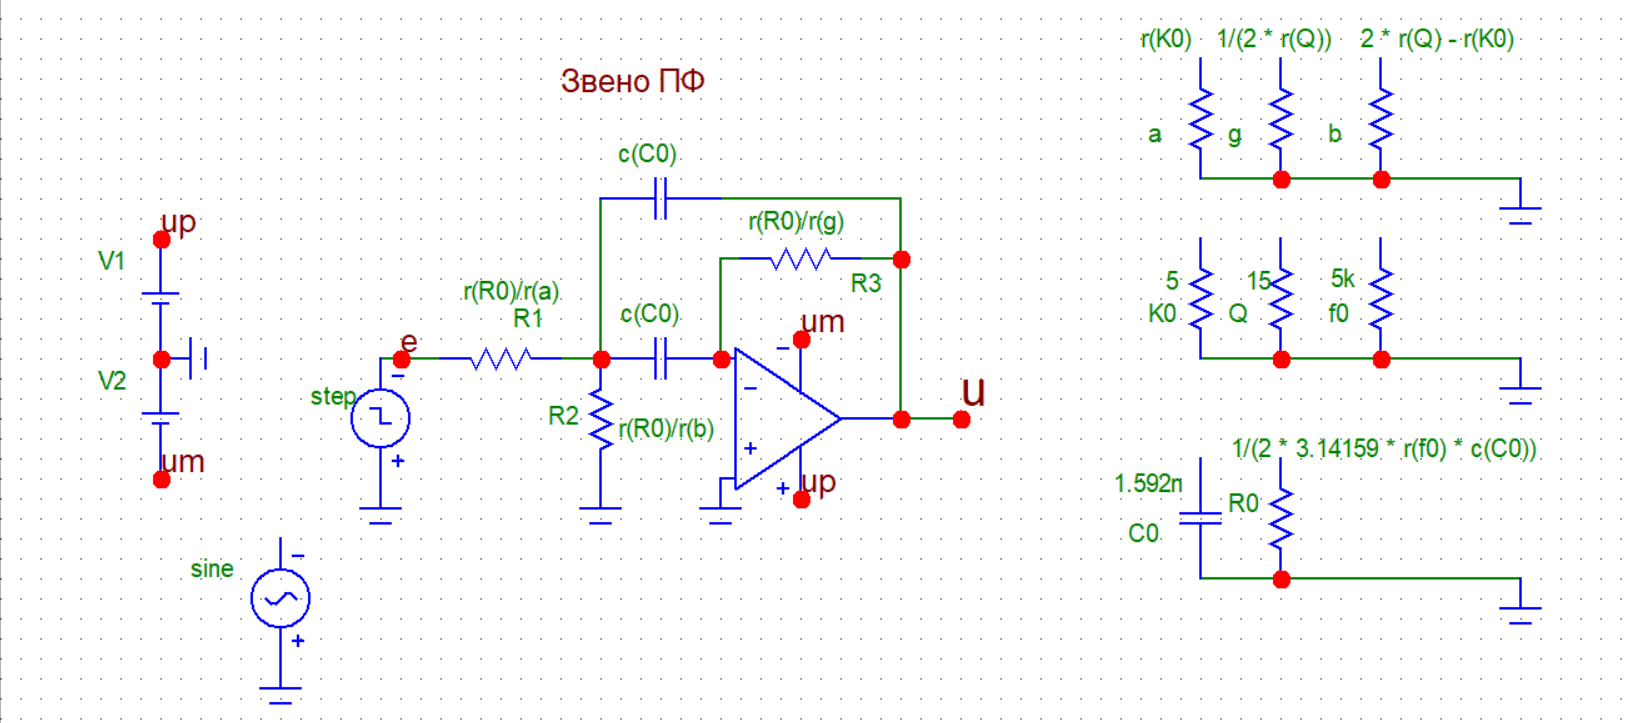
\includegraphics[width=1.0\linewidth]{res/amp1bp_scheme.png}
		\caption{Схема}
		\label{scheme}
	\end{figure}

	Сделаем полосовой фильтр с двойной обратной связью с параметрами $f_0 = 5k$, $K_0 = 5$, $Q = 15$.
	
	Ожидаемая ширина полосы пропускания $\Delta f = \frac{f_0}{Q} = 330$ Гц, высота пика $K_{max} = QK_0 = 75$.
	
	\begin{figure}[H]
		\centering
		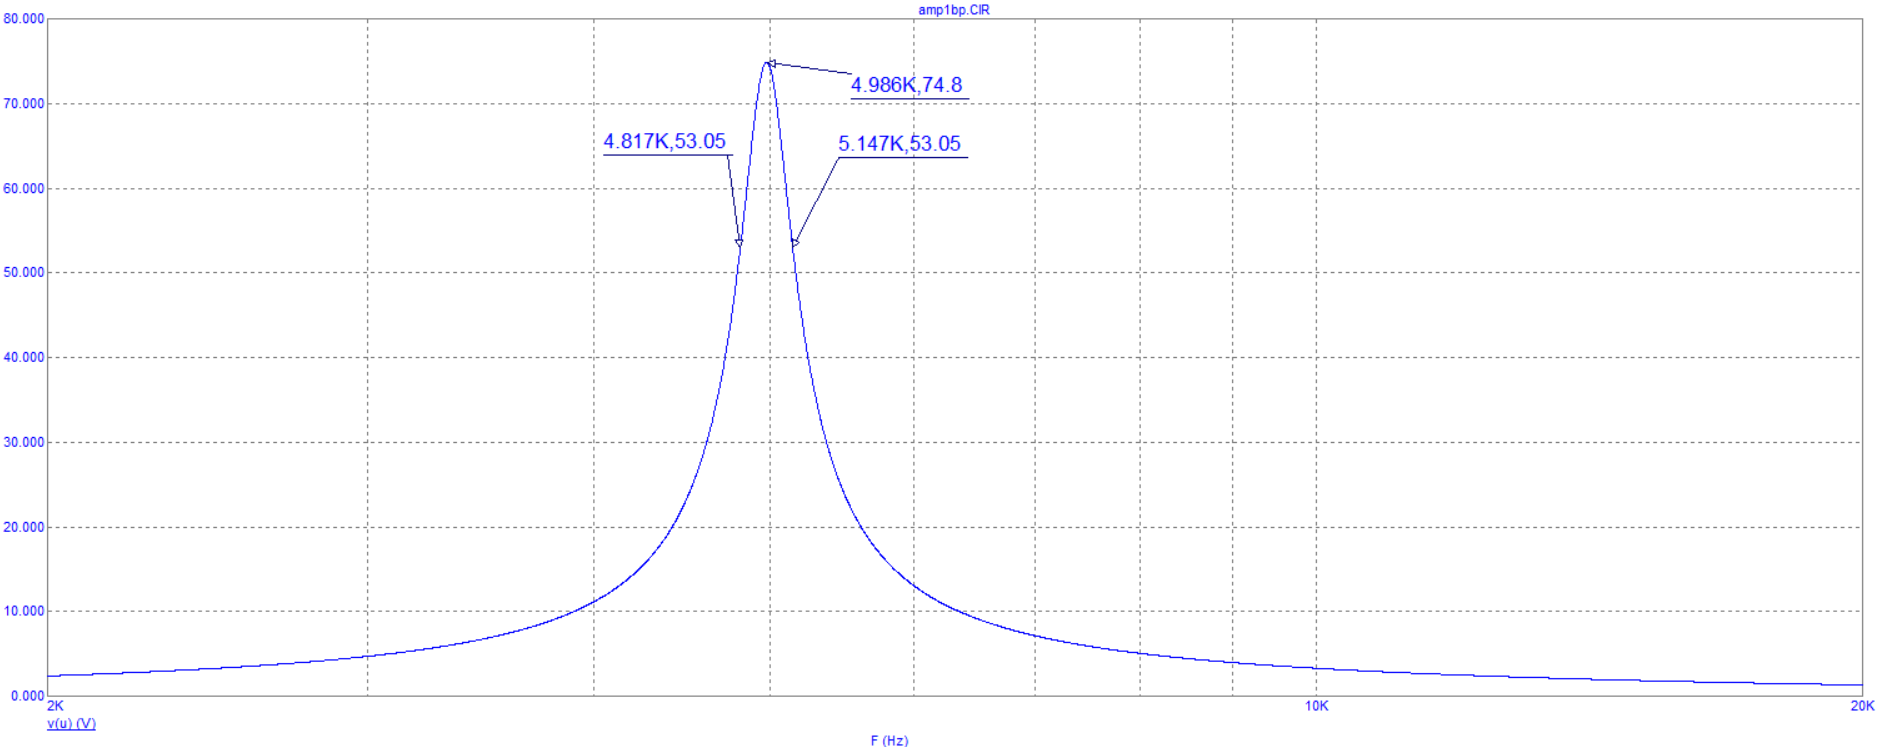
\includegraphics[width=1.0\linewidth]{res/amp1bp_ach.png}
		\caption{АЧХ фильтра}
		\label{ach}
	\end{figure}
	
	Как видно из графика, параметры совпадают с ожидаемыми.
	
	Проварьируем $R_2= [100, 1.3k | 200]$:
	\begin{figure}[H]
		\centering
		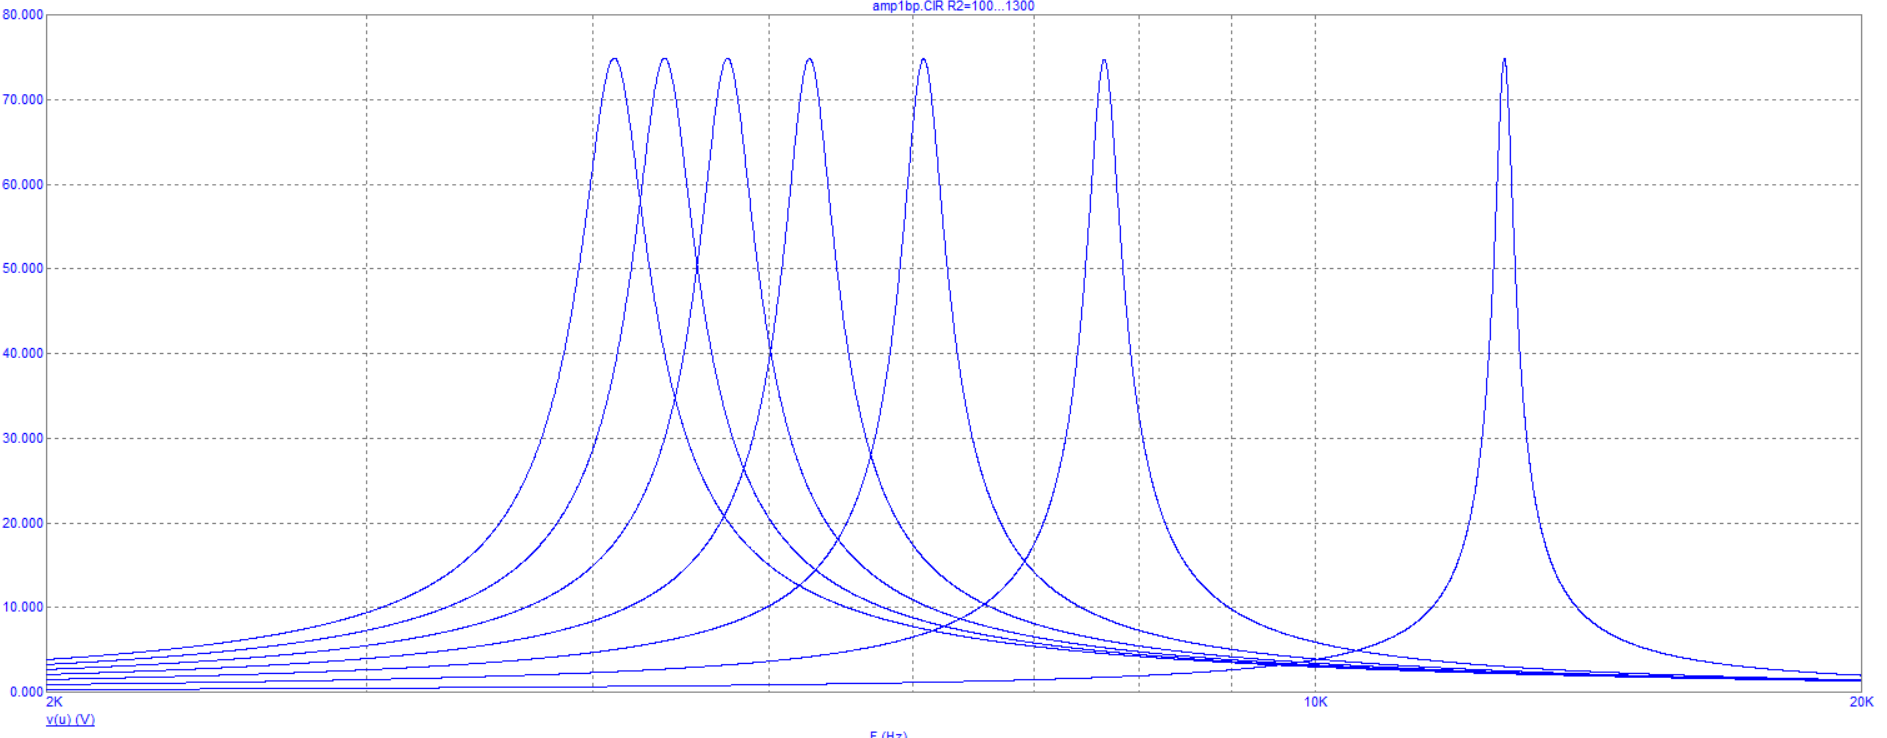
\includegraphics[width=1.0\linewidth]{res/amp1bp_R2.png}
		\caption{АЧХ от $R_2$}
		\label{ach}
	\end{figure}

	График зависимости частоты пика от $R_2$.
	\begin{figure}[H]
		\centering
		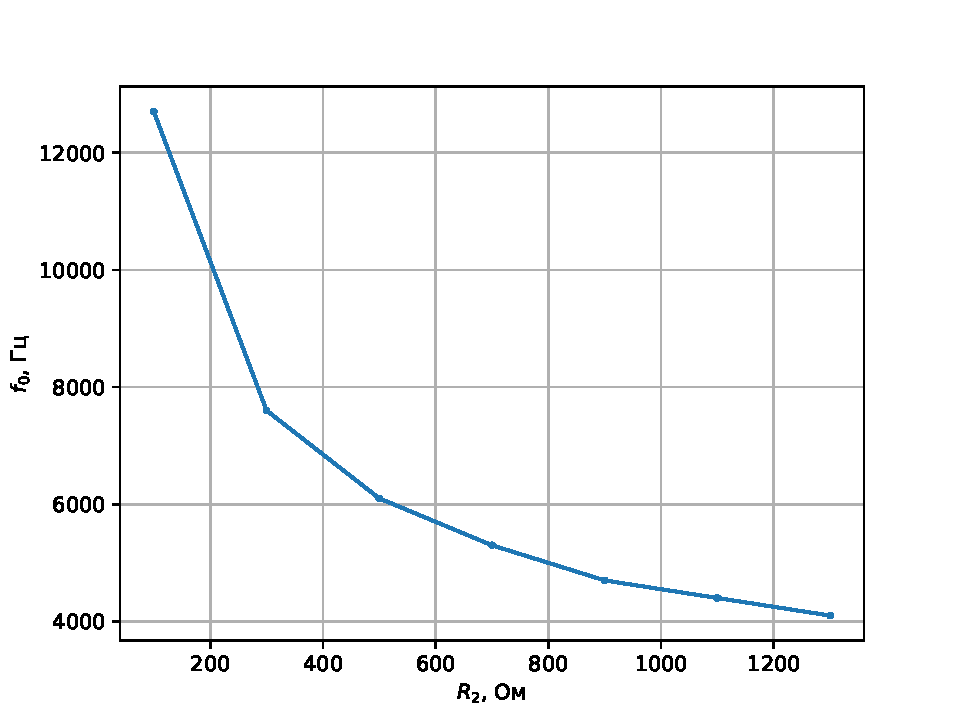
\includegraphics[width=0.8\linewidth]{res/amp1bp_R2.pdf}
		\caption{АЧХ от $R_2$}
		\label{ach}
	\end{figure}
	
	Соберем схему на макетной плате.
	
	\begin{figure}[H]
		\centering
		\begin{minipage}[b]{.5\textwidth}
				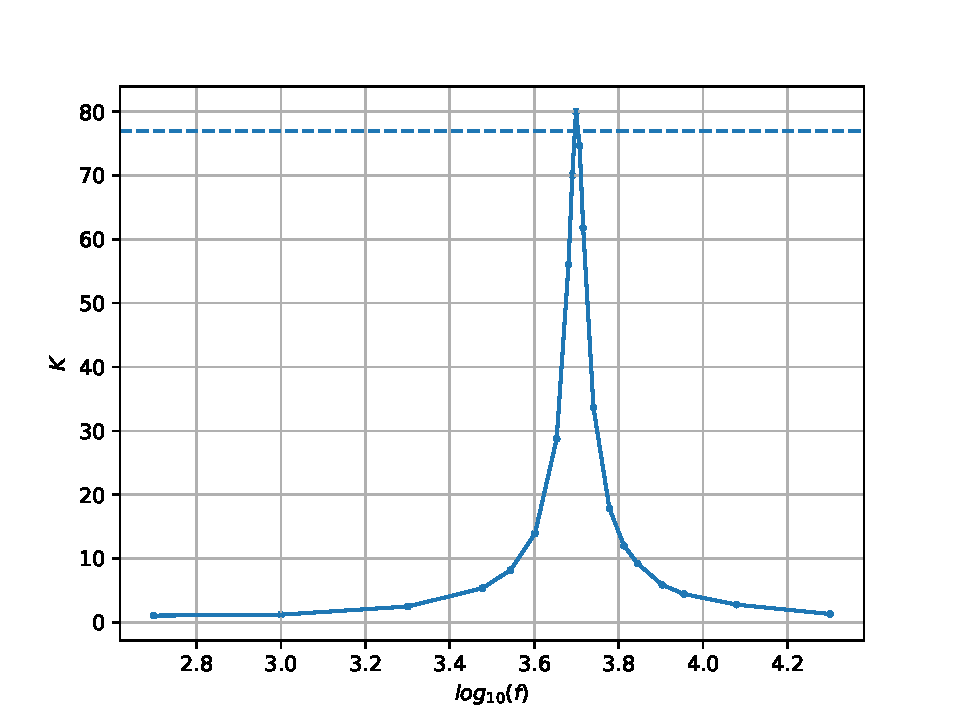
\includegraphics[width=1\linewidth]{res/amp1bp_ach.pdf}
			\end{minipage}%
		\begin{minipage}[b]{.5\textwidth}
				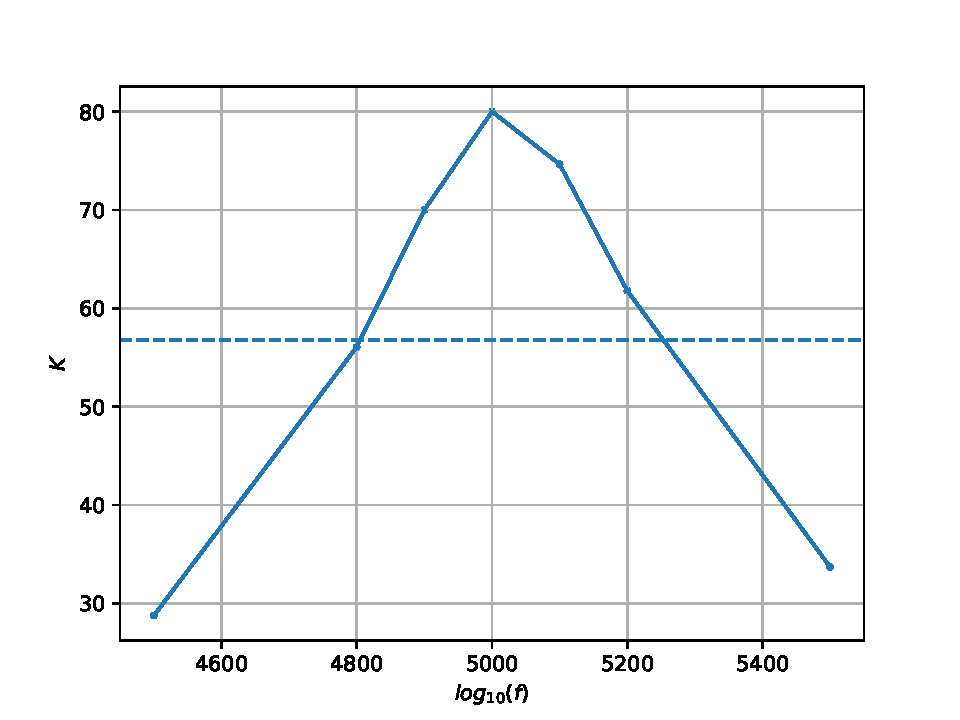
\includegraphics[width=1\linewidth]{res/amp1bp_achscoped.pdf}
			\end{minipage}
		\caption{АЧХ реального фильтра}
	\end{figure}
	
	Значения незначительно отклонились от ожидаемых.
	
	Соберем полосовой фильтр Чебышева третьего порядка с параметрами $f_0 = 1k$, $\varepsilon = 1$, $Q = \frac{f_0}{\Delta f} = 3$.
	
	Для получения параметров с помощью $MatLab$ получаем полюса: $(\nu_0, Q_0) = (1.0, 10.66), (\nu_1, Q_1) = (0.86, 20.36), (\nu_2, Q_2) = (1.162, 20.36)$.
	Коэффициенты усиления звеньев $K_0 = 1$.

	Реализуем с помощью ФНЧ полюс $(\nu_1, Q_1)$: $C^{*} = C \frac{1}{\nu_1} = 10n / 0.86 = 11.63n$, $a C = 3 Q_1 C^{*} = 710.36n$, $bC = \frac{C^{*}}{3 Q_1} = 0.19n$.
	
	С помощью ФВЧ реализуем $(\nu_2, Q_2)$: $R^* = R / \nu_2 = 10k / 1.162 = 8.61k$, $R / \alpha = \frac{R^*}{3Q_2} = 0.141k$, $R / \beta = 3Q_2 R^* = 525.9k$.
	
	Реализуем $(\nu_0, Q_0)$ с помощью ПФ: $R/\gamma = 2 * Q_0 * R = 213.2k$, $R/\beta = \frac{R}{2 Q_0 - 1} = 0.492k$.
	
	
	\begin{figure}[H]
		\centering
		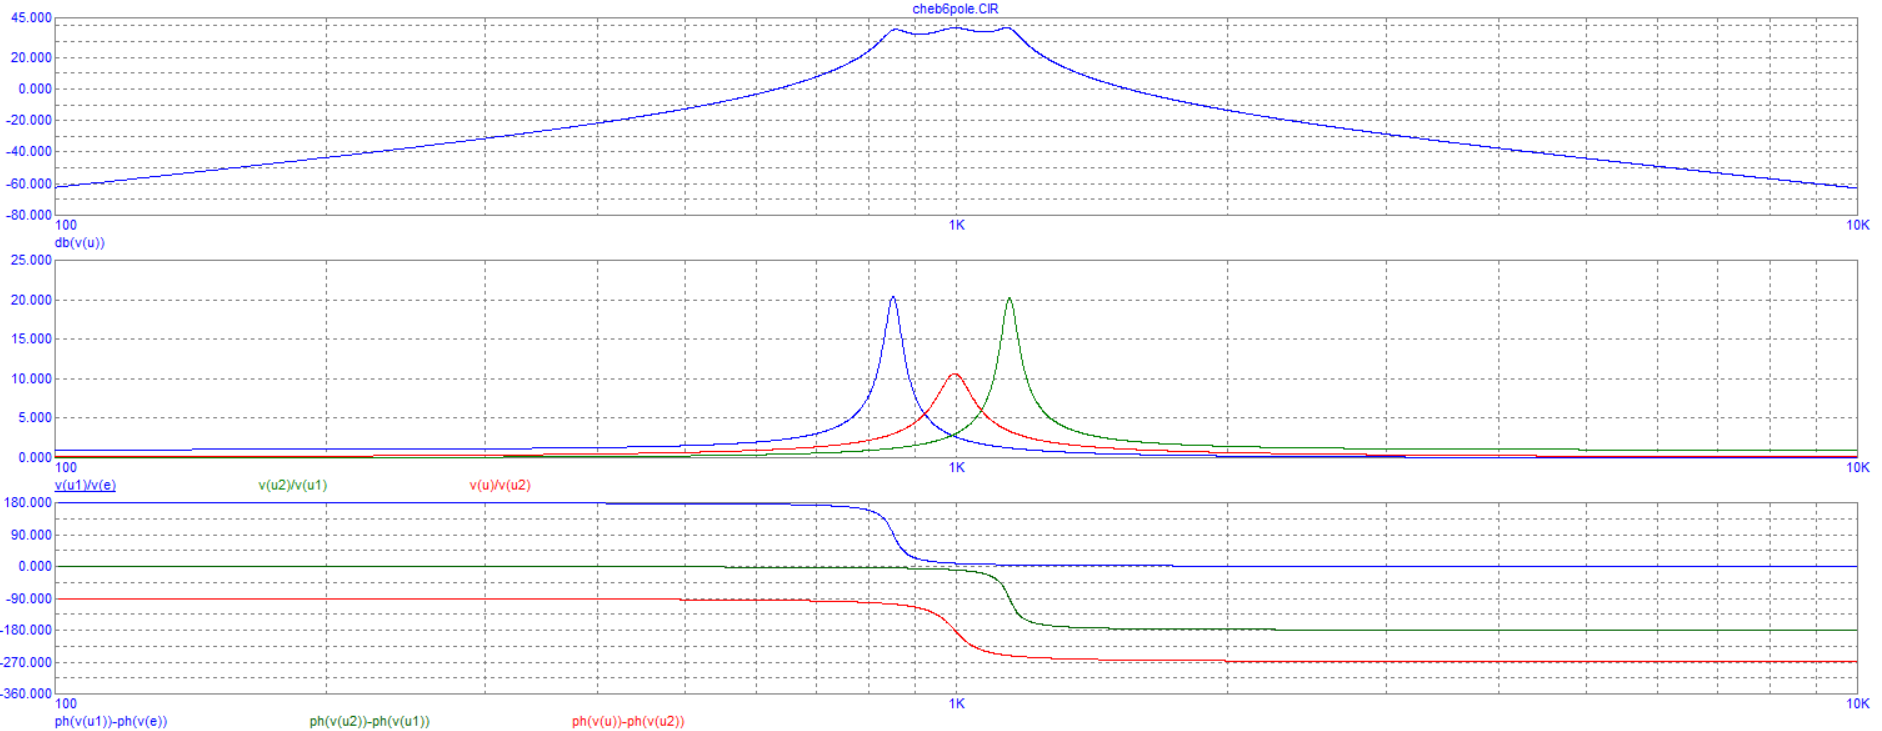
\includegraphics[width=1.0\linewidth]{res/cheb6pole.png}
		\caption{Фильтр Чебышева третьего порядка}
		\label{ach}
	\end{figure}
	
	\begin{figure}[H]
		\centering
		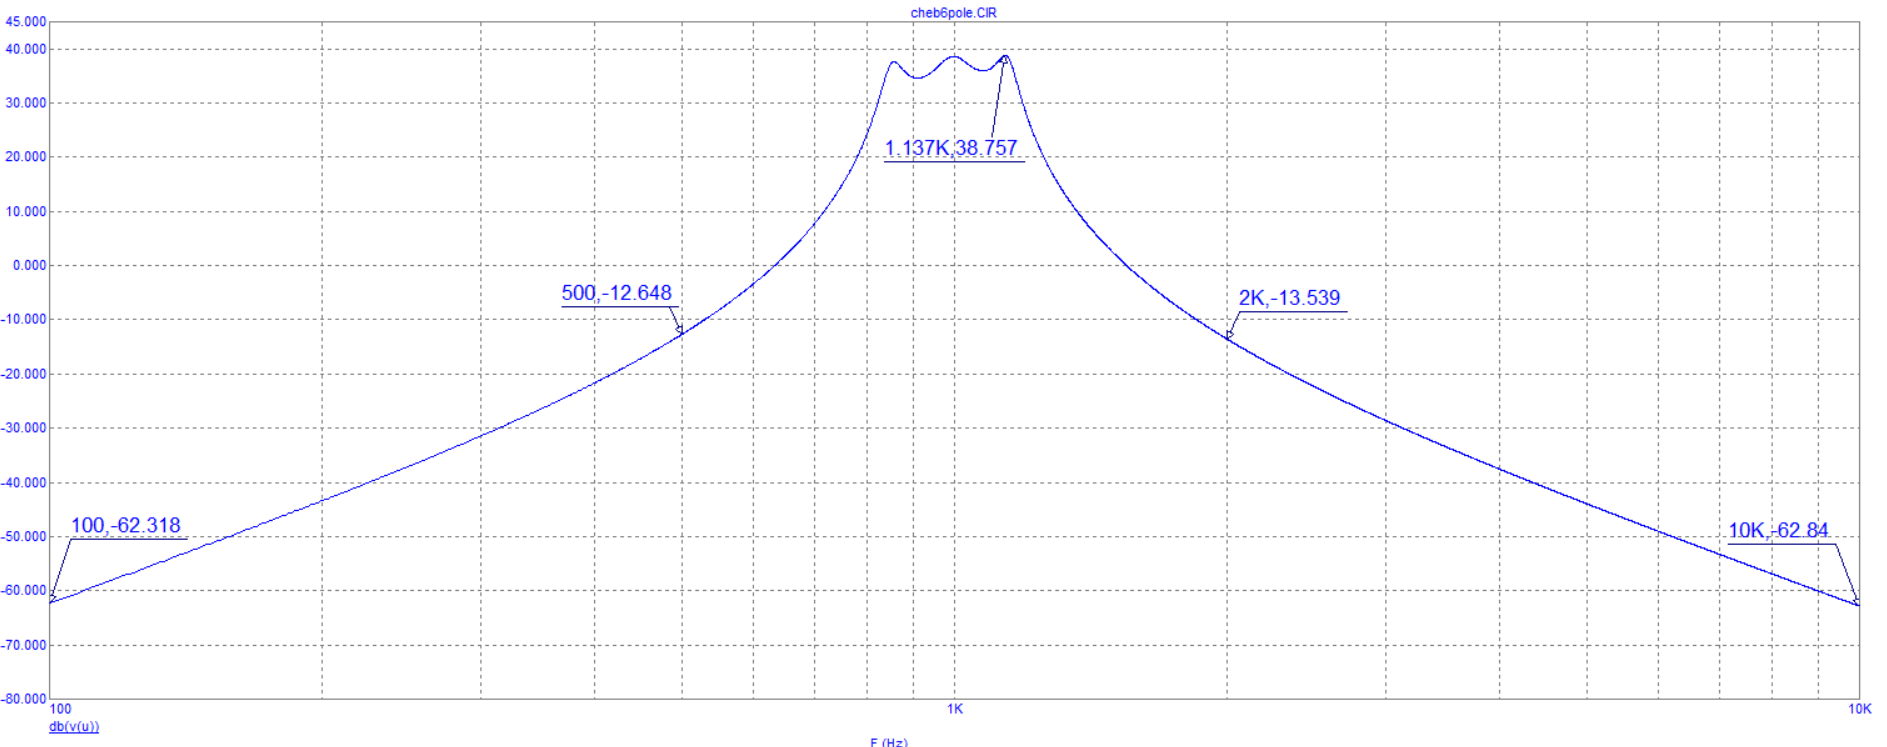
\includegraphics[width=1.0\linewidth]{res/cheb6pole_ach.png}
		\caption{АЧХ фильтра Чебышева третьего порядка}
		\label{ach}
	\end{figure}
	
	
%	Люблю своего Сашеньку. Не обижайте его!!! ^_^
	
\end{document}